\part{Algorithmische Mathematik 1}

\input{chapters/einführung}

\addchap{Zahlendarstellung am Computer}
\section{Zahlensystem}
Die Darstellung von Zahlen basiert auf sogenannten \emph{Zahlensystemen}.
Diese Zahlensysteme unterscheiden sich in der Wahl des zugrundeliegendes Alphabets.
Unsere Zahl entspricht dann einem Wort, bestehend aus Elementen des Alphabets.\\

\begin{definition}[Alphabet]
Es sei $\N = \{ 1,2,3\ldots \}$ und $b \in  \N$. \\
Wir bezeichnen mit $\sum_{b}$ das Alphabet des \emph{b-adischen Zahlensystems}
\end{definition}

\begin{example}
Verschiedene Zahlensysteme
\begin{enumerate}
	\item Dezimalsystem: $\sum_{10}= \{0,1,\ldots,9\}$ \\ wie $(384)_{10}$
	\item Dual bzw. Binärsystem $\sum_2 = \{0,1\}$ \\ wie $(42)_{10} = (101010)_2$
	\item Oktalsystem $\sum_8 = \{0,\ldots,7\}$ \\ wie $(42)_{10} = (52)_8$
	\item Hexadezimalsystem $\sum_{16} = \{0,\ldots,9,A,B,\ldots,F \}$ \\ wie $(42)_{10} = (2A)_{16}$
\end{enumerate}
\end{example}
Um die Zahlendarstellung sinnvoll zu nutzen Ergibt sich folgendes:
\begin{theorem}[]
Seien $b,n \in  \N, b>1 $. \\
Dann ist jede ganze, nicht-negative Zahl $z$ mit $0\le z \le b^{n}-1$ \emph{eindeutig} als Wort der Länge $n$ über $\sum_b$ darstellbar durch:
\[
z=\sum_{i=0}^{n-1}z_ib^{i}
\]
mit $z_i \in \sum_b$ für alle $i=0,1,\ldots,n-1$. \\
Wir schreiben vereinfachend: 
\[
z=(z_{n-1},\ldots, z_0)_b
\]
\end{theorem}
\begin{proof}

\begin{itemize}
\item Induktion \medskip
\begin{itemize}[label=$\lozenge$, itemsep=2ex]
\item \emph{Induktionsanfang}: \underline{$z<b$} hat die eindeutige Darstellung $z_0=z$ und $z_i=0$ sonst.



\item \emph{Induktionsschritt}: \underline{$z-1 \to z\ge b$} \\   

Betrachte
\[
z= \left\lfloor{\frac{z}{b}}\right\rfloor \cdot b + (z \mod b)
\]
Da $\hat{z}<z$ besitzt die eindeutige Darstellung
\[
\hat{z}= (\hat{z_{n-1}},\ldots, \hat{z_0})_b
\]
Bemerke $\hat{z_{n-1}}=0$, da 
\[
\left( \hat{z_{n-1}}b^{n-1} \right)b \le z \le b^{n}-1
\]
Also ist $z_b$ eine n-stellige Darstellung von z in b-adischen Zahlensystem

\end{itemize}

\item Eindeutigkeit wird durch Widerspruch gezeigt. \\
\emph{Angenommen:} Es gibt zwei verschiedene Darstellungen
\[
z=\left( z_{n-1}^{(2)},\ldots, z_0^{(2)} \right)_b = \left(z_{n-1}^{(1)},\ldots,z_0^{(1)} \right)_b
\]
Sei $m \in  \N$ der größte Index mit $z_m^{(1)} \neq z_m^{(2)}$, \\
Ohne Beschränkung der Allgemeinheit kann gesagt werden $z_m^{(1)>z_m^{(2)}}$. \\
Dann müssten die Stellen $0,1,\ldots,m-1$ den niedrigeren Wert von $z_m^{(2)}$ kompensieren. Die größte mit diesen Stellen darstellbare Zahl ist aber:
\[
\sum_{i=0}^{m-1}(b-1)b^{i}= (b-1)\sum_{i=0}^{m-1}b^{i}= b^{m}-1 \text{.}
\]
Da $b^{m}$ der kleinstmögliche Wert der fehlende Stelle m ist, kann diese aber nicht kompensiert werden. Dies ist ein Widerspruch.
\end{itemize}
\end{proof}%
Durch den Beweis ergibt sich sofort ein Algorithmus zur Umwandlung einer Zahl in ein anderes Zahlensystem:
\begin{example}
Umwandlung von $(1364)_{10}$ in das Oktalsystem.
\begin{itemize}
	\item $1364 = 170 \cdot 8 +4$
	\item $170 = 21 \cdot 8 +2$
	\item \ldots
	\item $0 \cdot 8 + 2$
\end{itemize}
$\implies (2524)_8$
\end{example}

\begin{algorithm}[H]
 \caption{Bestimmung der b-adischen Darstellung}
 \KwData{Dezimalzahl $z \in \N_0$, Basis $b \in \N$}
 \KwResult{b-adische Darstellung $(z_{n-1},\ldots, z_0)_b $}
 Initialisiere $i=0$ \\
 \While{$z>0$}{
  $z_i = z \mod b $\\
  $z= \left\lfloor \frac{z}{b} \right\rfloor$ \\
  $i=i+1$
 }
 \end{algorithm}

\paragraph{Beobachtung}
Wir sehen, dass das Honor-Schmea nur eine Schleife, Additionen und Multiplikationen benötigt. 
Diese Operationen können wir am Computer durchführen. 
Im Gegensatz dazu steht die Potenz $b^{i}$ in modernen Programmiersprachen zwar zur Verfügung, wird aber im Hintergrund oft auf Multiplikationen zurückgeführt.
Man überprüft leicht, dass das Honor-Schema weniger Multiplikationen benötigt und somit schnellt ist.

\section{Vorzeichen-Betrag-Darstellung}
Um auch Zahlen mit Vorzeichen am Computer darstellen zu können, betrachten wir im Folgenden die Vorzeichen-Betrag-Darstellung für Binärzahlen.
Das Binäralphabet besteht nur aus $0$ und $1$, welche wir auch als \emph{Bits} bezeichnen.
Bei einer Wortlänge von n Bits wir das erste Bit als Vorzeichen verwendet, die restlichen $n-1$-Bits für den Betrag der Zahl. Da die 0 die Darstellung $+0$ und $-O$ besitzt, können wir insgesamt $2^{n}-1$ Zahlen darstellen.

\begin{example}
Für $n=3$\\

\begin{table}[htpb]
	\centering
	\begin{tabular}{c c}
		Bitmuster & Dezimaldarstellung \\
		$000$ & $+0$ \\
		$001$ & $+1$ \\
		$\ldots$ & $\ldots$ \\
		$100$ & $-0$ \\
		$\ldots$ & $\ldots$ \\
		$111$ & $-3$
	\end{tabular}
\end{table}
\end{example}

\paragraph{Aber:} Diese Darstellung am Computer ist unpraktisch, da die vier Grundrechenarten auf Hardwareebene typischerweise mit Hilfe von Addition und Zusatz-Logik umgesetzt werden.
\paragraph{Lösung:} Komplementdarstellung

\section{Komplementdarstellung}

\begin{definition}[(b-1)-Komplement]
Sei $z=(z_{n-1}\ldots z_1 z_0)_b$ eine n-stellige b-adische Zahl. Das \emph{(b-1)-Komplement} $K_{b-1}(z)$ ist definiert als:
\[
K_{b-1} = (b-1-z_{n-1},\ldots, b-1-z_0)_b
\]
\end{definition}
Geben wir hierzu direkt ein paar Beispiele an
\begin{example} Komplemente \\
\begin{itemize}
	\item $K_9((325)_{10})= (674)_{10}$  (9er-Komplement im 10-er System)
	\item $K_1((10110)_2)=(01001)_2$ (1er-Komplement im 2er System)
\end{itemize}
\end{example}
\begin{definition}[b-Komplement]
Das b-Komplement einer b-adischen Zahl $z\neq 0$ ist definiert als \[
K_b(z)=K_{b-1}(z) +(1)_b
\]
\end{definition}
\begin{example}
\begin{itemize}
	\item $K_{10}((325)_{10}) = (674)_{10} + (1)_{10} = (675)_{10}$
\end{itemize}
\end{example}
\begin{lemma}[]
Für jede n-stellige b-adische Zahl $z$ gilt:
\begin{itemize}
	
	\item i) $z+K_{b-1}(z)=(b-1,\ldots,b-1)_b = b^{n}-1$
	\item ii) $K_{b-1}\left( K_{b-1}(z) \right)=z$
\end{itemize}
Ist außerdem $z\neq 0$ so gilt:
\begin{itemize}
	
	\item iii) $z+K_b(z)=b^{n}$
	\item iv) $K_b(K_b(z))=z$
\end{itemize}
\end{lemma}
\begin{proof}
\begin{itemize}Hilfssatz \\
	\item (i) Durch nachrechnen:
		\begin{align*}
		z+K_{b-1}(z)
		&=(z_{n-1} \ldots z_0)_b +(b-1-z_{n-1}, \ldots, b-1-z_0)_b \\
		&=\sum_{i=0}^{n-1}z_ib^{i}+ \sum_{i=0}^{n-1}(b-1-z_i)b^{i}\\
		&= \sum_{i=0}^{n-1}(b-1)b^{i} = (b-1, \ldots, b-1)_b \\
		&= (b-1)\sum_{i=0}^{n-1}b^{i} \\
		&=(b-1)\left( \frac{b^{n}-1}{b-1} \right) \\
		&= b^{n}-1
		\end{align*}
	\item (ii) per Definition
	\item (iii) Nachrechnen:
	\begin{align*}
		z+K_b(z) = z+K_{b-1} + 1 = b^{n}-1+1=b^{n}
	\end{align*}
	\item Definiere $\hat{z} = K_b\left( z \right)= K_{b-1}(z) + (1)_b > 0$ und rechne
		\[
		z+K_b(z)=b^{n}=\hat{z} +K_b{\hat{z}}+ K_b\left( K_b(z) \right) \implies \text{Behauptung.}
		\]
\end{itemize}



\end{proof}

\begin{remark} Modifikation 
\begin{itemize}
	\item Die 3. Aussage gilt auch für $z=0$, falls man dann bei der Addition von 1 die Anzahl der Stellen erweitert.
	\item die 4. Aussage gilt für $z=0$, falls überall im Beweis modulo $b^{n}$ gerechnet wird.
\end{itemize}
\end{remark}
Außerdem impliziert die 3. Aussage des Lemmas, dass 
\begin{equation}\label{eqn:komplement}
	K_b(z)=b^{n}-z \text{.}
\end{equation}
Dies können wir geschickt zum Darstellen der $b^{n}$ verschiedenen ganzen Zahlen $z$ mit 
\[
-\left\lfloor \frac{b^{n}}{2}\right\rfloor \le z \le \left\lceil \frac{b^{n}}{2}\right\rceil -1
\]
nutzen. Diesen Bereich nennt man darstellbaren Bereich.
\begin{definition}[b-Komplement-Darstellung]
	Die b-Komplement-Darstellung $(z)_{K_b} = (z_{n-1} \ldots z_0)_b$ einer Zahl $z \in  \Z$ im darstellbaren Bereich ist definiert als:
	\[
		(z)_{K_b}= \begin{cases}
			(z)_b & \text{falls } z \ge 0 \\
			\left( K_b(|z|) \right)_b & \text{falls } z<0
		\end{cases}
	\]
\end{definition}

\begin{example} Der darstellbare Bereich.
\begin{itemize}
	\item Sei $b = 10$, $n=2$. \\ 
Dann impliziert \eqref{eqn:komplement}, dass
\[
K_{10}(50)= 10^2-50=50
\]
\[
K_{10}(49)= 100 -49=51 \text{.}
\]
Der darstellbare Bereich ist nun 
\[
-50 \le z \le 49
\]
und hat konkrete Darstellungen:

\begin{center}
\begin{tabular}{ c c }
 Darstellung & Zahl   \\
 $0$ & $+0$  \\
 $1$ & $+1$ \\
 \ldots & \ldots \\
 $49$ & $+49$ \\
 $50$ & $-50$ \\
 \ldots & \ldots \\
 $99$ & $-1$
\end{tabular}
\end{center}

\item Sei $b=2$, $n=3$ Der darstellbare Bereich ist $-4 \le  z \le 3$. \\
\begin{center}
\begin{tabular}{ c c }
 Bitmuster & Dezimaldarstellung  \\ 
 $000$ & $0$   \\  
 $001$ & $1$  \\
 \ldots & \ldots \\
 $100$ & $-4$ \\
 \ldots & \ldots \\
 $111$ & $-1$
\end{tabular}
\end{center}
\end{itemize}
\end{example}%
Wir betrachten nun Addition und Subtraktion zweier Zahlen in b-Komplement-Darstellung. 
Hierzu bezeichne $(x)_{K_b} \oplus (y)_{K_b}$ die ziffernweise Addition der Darstellungen von x und y mit Übertrag ("schriftlich rechnen"), 
wobei ein eventueller Überlauf auf die $(n+1)$-te Stelle vernachlässigt wird (wir rechen also immer mit modulo $b^{n}$.
\begin{theorem}[Addition in b-Komplement-Darstelllung]
	Seien x und y zwei n-stellige, b-adische Zahlen und x,y und $x+y$ im darstellbaren Bereich.
Dann gilt:
\[
(x+y)_{K_b} = (x)_{K_b} \oplus (y)_{K_b}
\]
\end{theorem}
\begin{proof}
Wir betrachten dazu mehrere Fälle.
\begin{itemize}
	\item Fall $x,y \ge 0$: \\
\begin{align*}
(x)_{K_b} \oplus (y)_{K_b}
    &\overset{\text{Def.}}{=}\left( (x)_b + (y)_b \right) \mod b^{n} \\
    &\overset{\text{Def.}}{=} (x+y) \mod b^{n} \\
    &\overset{\text{Def.}}{=} (x+y)_{K_b} \\
\end{align*}
Der letzte Schritt ist möglich, da $(x+y)_{K_b}$ im darstellbaren Bereich sind.
\item Fall $x,y <0$
\begin{align*}
(x)_{K_b} \oplus (y)_{K_b}
&\overset{Def.}{=} \left( \left( K_b(|x|) \right)_b + \left( K_b(|y|) \right)_b \right) \mod b^{n} \\
&\overset{   }{=}\left( (K_b(|x|)) +\left( K_b\left( |x| \right) \right)\right) \mod b^{n} \\
&= (b^{n}-|x| + b^{n}-|y|) \mod b^{n} \\
&= (x+y) \mod b^{n} \\
&= (x+y)_{K_b}
\end{align*}
\item Fall $x\ge 0, y<0$: \\
\begin{align*}
(x)_{K_b} \oplus (y)_{K_b}
&\overset{Def.}{=} ((x)_b + (K_b(|y|))_b) \mod b^{n} \\
&=(x+K_b(|y|)) \mod b^{n} \\
&=(x+b^{n}-|y|) \mod b^{n} \\
&=(x+y) \mod b^{n} \\
&= (x+y)_{K_b}
\end{align*}
\item Fall $x<0, y\ge 0$: Analog
\end{itemize}
\end{proof}
\begin{theorem}[Subtraktion in b-Komplement-Darstellung]
	Seien x und y n-stellige b-adische Zahlen und x,y und x-y im darstellbaren Bereich.
	Dann gilt:
	\[
	(x-y)_{K_b} = (x)_{K_b} \oplus \left( K_b(y) \right)_{K_b}
	\]
\end{theorem}
\begin{proof}
\begin{itemize}
	\item Fall $y=0$ nichts zu zeigen.
	\item $y \neq 0$: \eqref{eqn:komplement} impliziert:
		\[
		-y=K_b(y) -b^{n}
		\]
	mit modulo $b^{n}$-rechnen folgt, dass
	\[
		(-y)_{K_b}= (K_b(y))_{K_b}
	\]
	ist und somit:
	\begin{align*}
		(x-y)_{K_b}
		&= (x+(-y))_{K_b} \\
		&= (x)_{K_b} \oplus (-y)_{K_b} \\
		&= (x)_{K_b} \oplus (K_b(y))_{K_b}	
	\end{align*}
\end{itemize}
\end{proof}
\begin{example}
Für $b=10$ und $n=2$ ist der darstellbare Bereich $-50 \le  z \le 49$
\begin{itemize}
	\item $(20+7)_{K_{10}} = (20)_{K_{10}} \oplus (7)_{K_{10}} =(27)_{K_{10}}=27$
	\item $28-5 = 28+ (-5)= (28)_{K_{10}} \oplus (95)_{K_{10}} = (23)_{K_{10}} =23 $
	\item $-18-20= (-18)+(-20) = \ldots = -28$
\end{itemize}
\end{example}
Die darstellbaren Zahlen kann man sich beim $K_b$-Komplement als Zahlenrad vorstellen.

%Hier muss eine coole Uhr eingefügt werden.

\paragraph{Achtung} Ein eventueller Überlauf bzw. Unterlauf wird im Allgemeinen nicht aufgefangen.
\begin{example}
In n-stelliger Binärarithmetik ist die größte darstellbare Zahl $x_{max} = (011\ldots 1)_{K_2}$ gleich  $2^{n-1}-1$. Hingegen ist $x_{max}+1=(100\ldots 0)_{K_2}$ und wir als $-2^{n-1}$ interpretiert.
\end{example}

\section{Fest-Komma-Darstellung}
\begin{definition}
	Bei der Festkommadarstellung einer n-stelligen Zahl werden k Vorkomma und n-k Nachkommastellen definiert:
	\[
	z=\pm (z_{k-1} \ldots z_0.z_{-1} \ldots z_{k-n})_b = \pm \sum_{i=k-n}^{k-1}z_i b^{i}
	\]

\end{definition}
\begin{example}
Im Zehner System wie gehabt.\\
Im Binärsystem ergibt sich folgendes: $(101.01)_2= 2^{2}+ 2^{0}+ 2^{-2}=5.25$
\end{example}
\paragraph{Achtung} Im Gegensatz zur Darstellung ganzer Zahlen können bereits bei der Konvertierung von Dezimalzahlen in das b-adische Zahlensystem Rundungsfehler auftreten.
\begin{example}
	$(0.8)_{10}=(0.110\overline{1100})_2$
\end{example}
Das größte Problem der Festkommadarstellung ist alllerdings, dass der darstellbare Bereich stark eingeschränkt ist und schlecht aufgelöst ist, da der Abstand zwischen zweier Zahlen immer gleich ist.
\begin{example}
Die kleinste darstellbare Zahl in Fixkommadarstellung ist \[
z_1=(0 \ldots 0.0 \ldots 0 1)_b
\]
Die zweitkleinste Zahl ist $z_2=2z_1$. Wir wollen $x=\frac{z_1+z_2}{2}$ in Fixkommadarstellung darstellen, müssen wir entweder zu $z_1$ abrunden oder zu $z_2$ aufrunden.
\end{example}
\begin{fluff}
Der relative Fehler dieses Runden ist:
\[
\frac{|x-z_1|}{|x|}=\frac{1}{3}
\]
Analog für $z_2$. \\
Solche Fehler machen jede Rechnung unbrauchbar.
\end{fluff}

\section{Gleitkommadarstellung}
\begin{definition}[Gleitkommadarstellung]
	Die Gleitkommastellung einer Zahl $z \in  \R$ ist gegeben durch:
	\[
	z=+-m\cdot b^{e}
	\]
mit einer \underline{Matisse} m, dem \underline{Exponenten} e und der \underline{Basis} b.
\end{definition}
Der Einfachheit halber nehmen wir an, dass die Basis für alle Zahlen gleich ist, obwohl sie prinzipiell verschieden sein könnte.
\begin{example}
Die Gleitkommadarstellungen von:
\begin{itemize}
	\item $(-384.753)_{10}= -3.84753 \cdot 10^2$
	\item $(0.00042)_{10}=4.2 \cdot 10^{-4d}$
	\item $(1010.101)_2= (1.010101)_2 \cdot 2^{3}$
\end{itemize}
\end{example}
\paragraph{Achtung:} Die Gleitkommadarstellung ist \underline{nicht} eindeutig!

\begin{definition}
Die Matisse m heißt \underline{normalisiert}, falls $m=m_1.m_2m_3 \ldots m_t$ mit $1\le m_1 \le b$.
\end{definition}
Um die eindeutige, normalisierte Gleitkommadarstellung im Computer zu speichern, müssen wir festlegen, wie viele Stellen für Matisse und Exponent zur Verfügung gestellt werden. Dies resultiert in der Menge 
\[
F=F(b,t,e_{min}, e_{max}) = \{z= +-m_1.m_2m_3\ldots m_t \cdot b^{e} | e_{min} \le e \le e_{max} \} 
\]
Da 0 nicht in dieser Form dargestellt werden kann, reserviert man dafür eine spezielle Ziffernfolge in Matisse und Exponent.
%Hier fehlt wieder ein schöne Grafik
\begin{remark}
Das Hidden Bit ist hilfreich
\begin{itemize}
	\item Für $b=2$ kann die erste Ziffer $m_1$ der Matisse weggelassen werden (Hidden Bit)
	\item Um den Exponenten besser vergleichen zu können, verwendet man oft die Exzess- oder Bias-Darstellung. Durch Addition der Exzesser $|e_{min}|+1$ wird der Exponetn auf den Bereich $1,2,\ldots, |e_{min}|+e_{max} +1 $ transformiert.
\end{itemize}
\end{remark}
\begin{example}[IEEE 754 Standard]
	Betrachte binäre Gleitkommazhalen mit 64 Bit auf dem Computer. 
	\begin{itemize}
		\item 52 Bit für die Matisse in Hidden Bit Darstellung
		\item 11 Bit für den Exponenten mit $e_{min} = -1022$ und $e_{max} =1023$ gespeichert in Exzessdarstellung.
		\item 1 Bit als Vorzeichen.
	\end{itemize}
Weiter Fälle können Online nachgelesen werden.
\end{example}

\subsubsection{Genauigkeit der Gleitkommadarstellung}
Da die Menge aller Zahlen in $F=F(b,t,e_{min},e_{max})$ endlich ist, müssen wir Zahlen in $\R \setminus  F$ geeignet annähern.

\begin{definition}
Die Rundung ist eine Abbildung $rd\colon \R \to F $ mit 
\begin{itemize}
	\item $rd(a)=a$, $a \in F$
	\item $rd(z)$, $z \in  \R$ ist gegeben so, dass $|z-rd(z)|=\underset{a \in F}{\min}(z-a)$ für alle $z \in  \R$.
\end{itemize}
\end{definition}
\begin{definition}[Maschinengenauigkeit]
Den maximalen relativen Rundungsfehler $\varepsilon_{mach}$ für $z_{min} \le |z| \le z_{max}$ nennt man Maschinengenauigkeit.
Die Stellen der Mantisse heißen \underline{signfikante Stellen}.
Wenn die Mantisse t-stellig ist, spricht man von \underline{t-stelliger Arithmetik}.
\end{definition}
\begin{theorem}[Maschinengenauigkeit von F]\label{thm:emach}
	Die Maschinengenauigkeit $\varepsilon_{mach}$ für $F=F(b,t,e_{min},e_{max})$ ist:
	\[
	\varepsilon_{mach} = \frac{1}{2} b^{1-t} \text{.}
	\]
\end{theorem}
\begin{proof}
Betrachte relativen Rundungsfehler $\varepsilon$, der vom Abscheiden nicht signifikanten Stellen herrüht. Sei $z_{min} < x < z_{max}$ und $\tilde{x}$ die durch Abschneiden entstehende Zahl.
Dann gilt:
\begin{align*}
	\varepsilon
	&= \frac{|x-\tilde{x}|}{|x|} \\
	&= \frac{|x_1.x_2x_3 \ldots x_t x_{t+1}\ldots \cdot b^{e}-x_1x_2x_3\ldots x_t \cdot b^{e}}{|x|} \\
	&=\frac{|0.x_{t+1}\ldots| \cdot |b^{e+1-t}|}{|x|}
\end{align*}
Da $|0.x_{t+1}\ldots|<1$ und $b^{e}\le |x|$ gilt:
\[
\varepsilon <\frac{b^{e+1-t}}{b^{e}}=b^{1-t}
\]
Da der Rundungsfehler $\varepsilon_{mach}$ höchsten halb so groß ist wie der Abschneidefehler folgt die Behauptung.
\end{proof}
Die Maschinengenauigkeit $\varepsilon_{mach}$ ist die wichtigste Größe zur Beurteilung der Genauigkeit von Gleitkommarechnungen am Computer. Sie gibt Aufschluss zur Anzahl signifikanter Stellen zur Basis $b$.
Die zugehörige Anzahl $s$ Stellen im Dezimalsystem erhält man durch das Auflösen von:
\[
\varepsilon_{mach} = \frac{1}{2}b^{1-t}=\frac{1}{2}10^{1-s}
\]
nach s. Es folgt daher:
\[
s= \lfloor 1+(t-1)\log_{10}(b) \rfloor
\]
Für den IEEE 754 Standard mit $b=2, t=53$ erhält man $s=16$ signifikante Stellen.


\addchap{Fehleranalyse}
\section{Rechnerarithmetik}
\begin{example}
Betrachte $F=F(10,5,-4,5)$ und Maschinenzahlen
\begin{align*}
x=2.5684 \cdot 10^{0}= 2.56840000 \\
y=3.2791 \cdot 10^{-3} = 0.0032791
\end{align*}
Es gilt:\\
\begin{center}
$\begin{rcases}
	x+y= 2.5716792 \\
	x-y= 2.5651209 \\
	x \cdot y= 0.00842204044 \\
	\frac{x}{y}= 783.2637004
\end{rcases} \not\in F$
\end{center}
\end{example}
\begin{remark}
Die Menge $F(b,t,e_{min},e_{max})$ ist nicht abgeschlossen bezüglich der Grundrechenarten und können somit im Allgemeinen nicht im Computer implementiert werden.
\end{remark}
\paragraph{Lösung}
Wir runden das Ergebnis und implementieren so eine Pseudoarithmetik.
Das bedeutet, wir ersetzen $\circ \in  \{+,-,\cdot, \div\}$ durch $\boxcircle \in \{\boxplus, \boxminus, \boxdot, \boxslash\}$ definiert durch:
\begin{equation}\label{eqn:rundung}
x \boxcircle y \coloneqq rd (x \circ y)
\end{equation}
Auf Hardwareebene wird üblicherweise mit einer längeren Matisse gearbeitet und dann normalisiert und gerundet. Dies entspricht dem IEEE 754 Standard.
\begin{remark}
Für $|x|,|y|, |x \circ y| \in [z_{min},z_{max}]$ impliziert \eqref{eqn:rundung}, dass
\[
	\frac{|x \boxcircle y - x \circ y|}{|x \circ y|}= \frac{rd(x \circ y - x \circ y)}{|x \circ y|} \le \varepsilon_{mach}
\]

Das bedeutet, dass $\boxcircle$ im Computer bestmöglich umgesetzt ist.
\end{remark}
\begin{example}
Betrachte $F=F(10,5,-4,5)$ \\
\begin{itemize}
	\item Setze:
\begin{itemize}
	\item $a=0.98765$
	\item $b=0.012424$
	\item $c=-0.0065432$
\end{itemize}
Dann gilt:
\[
	(a+b)+c=a+(b+c)=0.9925208
\]
Numerisch gilt:
\[
(0.98765 \boxplus 0.012424)\boxminus 0.0065432= rd(0.9935568)=0.99356
\]
und
\[
0.98765 \boxplus (0.012424\boxminus 0.0065432)=rd(0.9935308)=0.99353
\]
\item Setze
	\begin{itemize}
		\item $a=4.2832$
		\item $b=-4.2821$
		\item $5.7632$
	\end{itemize}
Dann gilt
\[
(a+b)\cdot c = a \cdot c + b \cdot c = 0.006339520000001
\]
Numerisch gilt:
\end{itemize}
\end{example}
\begin{remark}
Mathematisch äquivalente Algorithmen auf Fließkommazahlen können je nach Implementierung zu wesentlich unterschiedlichen Ergebnissen führen, selbst wenn die Eingangszahlen exakt dargestellt werden.
\end{remark}
\subsection{Auslöschung}
Unglücklicherweise pflanzen sich numerische Fehler, zum Beispiel durch Rundung im Verlauf eines Algorithmus fort.

\begin{lemma}[Fehlerfortpflanzung]
Es seien $x,y \in \R$ mit Datenfehlern $\Delta x, \Delta y \in  \R$ behaftet, welche\[
|\frac{\Delta x}{x}| , |\frac{\Delta y}{y}| \ll 1
\]
erfüllen. Für $\circ \in  \{+,-,\cdot, \div\}$ gilt für den fortgepflanzten Fehler
\[
\Delta (x \circ y) \coloneqq (x+ \Delta x) \circ (y + \Delta y) - x \circ y \text{, }
\]
dass
\begin{equation*}
\begin{split}
\frac{\Delta (x \pm y)}{x \pm y} = \frac{x}{x \pm y}\frac{\Delta x}{x} \pm \frac{y}{x \pm y} \frac{\Delta y}{y} \\
\frac{\Delta (x \cdot y)}{xy} \approx \frac{\Delta x}{x}+ \frac{\Delta y}{y} \\
\frac{\Delta (\frac{x}{y})}{\frac{x}{y}} \approx \frac{\Delta x}{x}-\frac{\Delta y}{y}
\end{split}
\end{equation*}
Hierbei bedeutet "$\approx$", dass Terme mit $(\Delta x)^2, (\Delta y)^2, \Delta x \Delta y$ vernachlässigt werden.
\end{lemma}
\begin{proof}
Übung.
\end{proof}
Für $\cdot,\div$ addieren bzw. subtrahieren sich die Fehler.
\paragraph{Achtung:} Ist $|x \pm y|$ wesentlich kleiner als $|x|$ oder $|y|$, kann der relative Fehler massiv verstärkt werden. 
Dieses Phänomen heißt Auslöschung.\\
Bei der Konstruktion von Algorithmen sollte Auslöschung möglichst vermieden werden.
\begin{example}\label{eg:pq}
Betrachte \\
\begin{equation}
\label{eqn:pq}
x^2-2px+q=0
\end{equation}
mit Lösungen:
\[
x_{1,2} = p \pm \sqrt[2]{p^2-q} 
\]


\begin{algorithm}[H]
 \label{alg:nst1}
 \caption{naive Nullstellenberechung}
 \KwData{$p,q \in \R$ so ,dass \eqref{eqn:pq} lösbar ist}
 \KwResult{Nullstellen $x_1,x_2$ von \eqref{eqn:pq}.}
 $d=\sqrt{p\cdot p -q}$ \\
 $x_1= p+d$ \\
 $x_2= p-d$
 \end{algorithm}
 Mit $p=100$, $q=1$ in dreistelliger, dezimaler Gleitkommaarithmetik ergibt sich:
 \begin{equation*}
	 \begin{split}
		 d= \sqrt{10000-1}= \sqrt{rd(9999)}=\sqrt{10000} = 100 \\
		 x_1=100+100=200 \\
		 x_2= 100-100 =0
	 \end{split}
 \end{equation*}
Die exakten Werte sind  $x_1 \approx 199.99, x_2 \approx 0.00500$, welche in dreistelliger, dezimaler Gleitkommaarithmetik als $x_1=200,x_2=0$ dargestellt werden. \\
Gemäß \ref{thm:emach} ist die Maschinengenauigkeit:
\[
\varepsilon_{mach} = \frac{1}{2}b^{1-t}= \frac{1}{2}10^{1-3}=0.005
\]
Der relative Fehler $\frac{|0-0.005|}{|0.005|}=1$ ist also zu 100 Prozent falsch.
\end{example}
Wir können die Genauigkeit von $x_2$ erhöhen, indem wir den Wurzelsatz von Vieta $x_1x_2=q$ verwenden.\\
\begin{algorithm}[H]
 \caption{verbesserte Nullstellenberechnung}
 \KwData{$p,q \in  \R$ so ,dass \eqref{eqn:pq} lösbar ist.}
 \KwResult{Nullstellen $x_1,x_2$ \eqref{eqn:pq}.}
 $d= \sqrt[2]{p \cdot p -q}$ \\
 \If{$q \ge 0$}{$x_1=p+d$
 \Else{$x_1=p-d$}}
 $x_2=\frac{q}{x_1}$
 \end{algorithm}
 Wir erhalten nun $d=100, x_1=200,x_2=\frac{1}{200}=0.005$

\section{Vorwärts- und Rückwertsanalyse}
Abstrakt gesehen entspricht das Lösen eines Problems dem Auswerten einer Funktion $f$.
Beim numerischen Auswerten von $f$ können verschiedene Fehler passieren:
%Hier muss noch das Diagramm von Vorlesung 5 hin.

\begin{definition}[Fehlerarten]
Sei $D \subset \R$ eine Menge von Eingangsdaten und $W \subset \R$ die Menge der möglichen Ergebnisse. Wir unterscheiden folgende Fehlerarten bei der Auswertung von $f \colon D \to W$.
\begin{itemize}
\item \underline{Datenfehler} Typischerweise sind die Eingangsdaten $x \in D$ nicht exakt,
sondern mit einem Datenfehler $\Delta x$ behaftet. Die gestörten Eingangsdaten $\tilde{x}=x+ \Delta x$ produzieren einen Fehler $f(x+\Delta x)-f(x)$.
\item \underline{Verfahrensfehler} Exakte Verfahren enden bei exakter Rechnung nach endlich vielen Operationen mit dem exakten Ergebnis.
Näherungsverfahren enden in Abhängigkeit bestimmter Kriterien mit einer Näherung $\tilde{y}$ für die Lösung $y \in W$.
\item \underline{Rundungsfehler} Verursacht durch Maschinenzahlen und Rundungen während der Arithmetik.
\end{itemize}
\end{definition}
Ein Teilgebiet der Numerik versucht diese Fehler durch eine Fehleranalyse zu quantifizieren.
Hierzu verfolgt man die Auswirkungen von allen Fehlern, die in den einzelnen Schritten vorkommen können.
\begin{definition}[Analysearten]
Bei der \emph{Vorwärtsanalyse} wird der Fehler von Schritt zu Schritt verfolgt und der akkumulierte Fehler für jedes Teil-Ergebnis abgeschätzt. \\
Bei der \emph{Rückwertsanalyse} geschieht die Verfolgung des Fehlers hingegen so, dass jedes Zwischenergebnis als exakt berechnetes Ergebnis zu gestörten Daten interpretiert wird, d.h , der akkumulierte Fehler wird als Datenfehler interpretiert.
\end{definition}
\begin{example}
Betrachte $f(x,y)=x+y$ \\
\begin{itemize}
	\item Vorwärtsanalyse: $\boxed{f} = x \boxplus y= (x+y)(1+\varepsilon)$
	\item Rückwärtsanalyse: $x \boxplus y= x(1+\varepsilon)+y(1+\varepsilon)= f(x(1+\varepsilon), y(1+\varepsilon))$
\end{itemize}
mit $|\varepsilon|\le \varepsilon_{mach}$
\end{example}
In der Praxis ist die Vorwärtsanalyse kaum durchführbar. 
Für die meisten Algorithmen ist, wenn überhaupt, nur eine Rückwärtsanalyse bekannt.
\begin{example}
\label{eg:rückwärtsanalyse}
Fortsetzung von Beispiel \ref{eg:pq} \\
Führe Rückwärtsanalyse durch zu Algorithmus \ref{alg:nst1} für die Betrags-kleinere Nullstelle $x_2$ durch:
Dann ist
\[
f(p,q)=p-\sqrt[2]{p^2-q}
\]
mit $p>0$. 
Für $|\varepsilon_i|\le \varepsilon_{mach}, i=1,2,3,4$ betrachten wir:
\begin{align*}
\left( p-\sqrt[2]{(p^2(1+\varepsilon_1)-q)(1+\varepsilon_2)} (1+\varepsilon_3) \right)(1+\varepsilon_4)
&= p(1+\varepsilon_4)-\sqrt[2]{(p^2(1+\varepsilon_1)-q)(1+\varepsilon_2)(1+\varepsilon_3)^2(1+\varepsilon_4)^2}\\
&= p^2(1+\varepsilon_1)(1+\varepsilon_3)^2(1+\varepsilon_4)^2-q(1+\varepsilon_2)(1+\varepsilon_3)^2(1+\varepsilon_4)^2 \\
&= \ldots \\
&= p(1+\varepsilon_4)-\sqrt[2]{p^2(1+\varepsilon_4)^2-q(1+\varepsilon_7)} \\
&= f(p(1+\varepsilon_4),q(1+\varepsilon_7))
\end{align*}
Die Abschätzung für $\varepsilon_7$ explodiert, falls $0<|q| \ll 1 < p$. Dies war in Beispiel \ref{eg:pq} der Fall.
\end{example}

\input{chapters/sections-alma1/kondition-stabilität}

\addchap{Dreitermrekursion}
\section{Theoretische Grundlagen}
\begin{definition}
Für gegebene $p_0$ und $p_1$ heißt eine Rekursion der Form
\begin{equation}
	\label{eqn:dreitermrekursion}
	p_k=a_kp_{k-1}+b_kp_{k-2}+c_k\text{, } k=2,3,\ldots
\end{equation}
mit $b_k\neq 0$ eine \emph{Dreitermrekursion}. Die zugehörige \emph{Rückwärtsrekursion} ist
\begin{equation}
	\label{eqn:rrekursion}
p_{k-2}= -\frac{a_k}{b_k}p_{k-1}+\frac{1}{b_k}p_k-\frac{c_k}{b_k}\text{, } k=n,n-1,\ldots
\end{equation}
Ist $b_k=1$, das heißt \eqref{eqn:dreitermrekursion} und \eqref{eqn:rrekursion} gehen durch vertauschen von $p_{k-2}$ und $p_k$ auseinander hervor, so heißt die Rekursion \underline{symmetrisch}. Gilt $c_k=0$ für alle $k$, so heißt die Rekursion \underline{homogen}.
\end{definition}
\begin{example}
Die Fibonacci-Zahlen sind rekursiv definiert durch:
\[
p_k=p_{k-1}+p_{k-2}
\]
mit $p_0=0, p_1=1$. Es gilt $a_k=b_k=1$. \\
Sei
\[
p_k(x)= 2\cos(x)p_{k-1}(x) -1 \cdot p_{k-2}(x)
\]
mit $p_0=1$ und $p_1=\cos(x)$. Man kann zeigen, dass
\[
p_k(x)=2\cos(kx)
\]
ist. \\
Die Chebychev-Polynome $T_k$ erfüllen 
\[
T_k(x)=2x T_{k-1} -T_{k-2}(x)
\]
mit $T_0(x)=1$ und $T_1(x)=x$
\end{example}

\begin{algorithm}[H]
\label{alg:rekursion}
 \caption{Dreitermrekursion}
 \KwData{Koeffizienten von $\{a_k\}_{k=2}^{n}$, $\{b_k\}_{k=2}^n$,$\{c_k\}_{k=2}^n$, Startwerte $p_0,p_1$}
 \KwResult{Werte von $\{p_k\}_{k=2}^n$}
\For{$k\gets 2$ \KwTo $n$}{
$p_k=a_kp_{k-1}+b_kp_{k-2}+c_k$
    }
 \end{algorithm}
 \begin{example}
	 \label{eg:rekursion}
 Betrachte: $p_0=1, p_1=\sqrt[2]{2}-1, p_k= -2p_{k-1}+p_{k-2}$, $k=2,3,\ldots$ \\
 Algorithmus \ref{alg:rekursion} liefert:

 %Nice Grafik

Die Oszillationen für höhere k sollten uns misstrauische machen und uns motivieren das Problem genauer anzuschauen.
 \end{example}
Wir können homogene Dreitermrekursion schreiben als:
\[
\begin{bmatrix}
	p_k \\
	p_{k-1}
\end{bmatrix}= \begin{bmatrix}
a_kp_{k-1} + b_kp_{k-2} \\
p_{k-1}
\end{bmatrix} \eqqcolon \begin{bmatrix}
a_k & b_k \\
1 & 0
\end{bmatrix} \cdot \begin{bmatrix}
p_{k-1} \\
p_{k-2}
\end{bmatrix} = A_k \begin{bmatrix}
p_{k-1} \\
p_{k-2}
\end{bmatrix}
\]
Rekursiv folgt:
\[
\begin{bmatrix}
p_k \\
p_{k-1}\end{bmatrix} = A_k \begin{bmatrix}
p_{k-1} \\
p_{k-2}
\end{bmatrix}= A_k A_{k-1} \begin{bmatrix}
p_{k-2} \\
p_{k-3}
\end{bmatrix}= \ldots = A_k \ldots A_2 \begin{bmatrix}
p_1 \\
p_0
\end{bmatrix}
\]
Offensichtlich gilt für alle $\alpha, \beta \in \R$ und Startwerte $p_0,p_1,q_0,q_1$ und $B_k \coloneqq A_k \ldots A_2$, dass
\[
B_k \begin{bmatrix}
\alpha p_1 + \beta q_1 \\
\alpha p_0 + \beta q_0
\end{bmatrix} = \alpha B_k \begin{bmatrix}
p_1 \\
p_0
\end{bmatrix} + \beta B_k \begin{bmatrix}
q_1 \\
q_0
\end{bmatrix}= \alpha \begin{bmatrix}
p_k \\
p_{k-1}
\end{bmatrix} + \beta \begin{bmatrix}
q_k \\
q_{k-1}
\end{bmatrix}
\]
Das heißt, die Lösungsfolge $\{p_k\}$ hängt \emph{linear} von den Startwerten
$\begin{bmatrix}
p_1 \\
p_0
\end{bmatrix} \in \R^2$ ab.
Im Falle unseres Beispiels gilt: $a_k=a=-2$, $b_k=b=1$. Das bedeutet, es gilt:
\[
B_k= A^{k-1}, A= \begin{bmatrix}
	a & b \\
	1 & 0
\end{bmatrix} = \begin{bmatrix}
	-2 & 1 \\
	1 & 0
\end{bmatrix}
\]
Aus den Eigenwerten $\lambda_1, \lambda_2$ der Matrix A kann man die Lösungen der homogenen Dreitermrekursion direkt angeben.
\begin{theorem}
	\label{thm:nst-polynom}
	Seien $\lambda_1, \lambda_2$ die Nullstellen des \emph{charakteristischen Polynoms}
	\begin{equation}
	\label{eqn:charpolynom}
	q(\lambda) = \lambda^2 -a \lambda -b
	\end{equation}
Dann ist die Lösung der homogenen Dreitermrekursion:
\[
p_k=ap_{k-1} +bp_{k-2}, k=2,3,\ldots
\]
gegeben durch:
\[
p_k= \alpha \lambda_1^{k}+\beta \lambda_2^{k}, k=2,3,\ldots
\]
mit $\alpha, \beta \in \R$ Lösungen des linearen Gleichungssystems.
\[
\alpha + \beta =p_0
\]
\[
\alpha \lambda_1 + \beta \lambda_2 =p_1
\]
\end{theorem}
\begin{proof}
\begin{itemize}
	\item Induktion über k\medskip
\begin{itemize}[label=$\lozenge$, itemsep=2ex]
\item Induktionsanfang: \underline{$k=0$}: 
	$p_0=\alpha+\beta = \alpha \lambda_1^{0}+\beta \lambda_2^{0}$
\item Induktionsschritt: \underline{$k \to k+1$}:
	\begin{align*}
	p_{k+1}
	&=ap_k +bp_{k-1} \\
	&= a(\alpha \lambda_1^{k}+ \beta \lambda_2^{k}) + b(\alpha \lambda_1^{k-1}+\beta \lambda_2^{k-1}) \\
	&= \alpha (a \lambda_1^{k}+ b\lambda_1^{k-1})+ \beta (a \lambda_2^{k}+ b \lambda_2^{k-1}) \\
	&= \alpha \lambda_1^{k-1}(a\lambda_1+b) + \beta \lambda_2^{k-1}(a\lambda_2 +b)\\
	&= \alpha \lambda_1^{k+1} + \beta \lambda_2^{k+1}
	\end{align*}
\end{itemize}
Da nach \eqref{eqn:charpolynom} $\lambda_1^2$ und $\lambda_2^2$ Nullstellen sind.
\end{itemize}
\end{proof}
Wende \ref{thm:nst-polynom} auf das Beispiel \ref{eg:rekursion} an: Mit $a=-2, b=1$ hat das charakteristische Polynom \eqref{eqn:charpolynom} die Nullstellen:
\[
\lambda_1= \sqrt[2]{2}-1, \lambda_2= -\sqrt[2]{2}-1 
\]
Aus
\[
\alpha + \beta =p_0 =1
\]
\[
\alpha \lambda_1 + \beta \lambda_2= p_1 = \sqrt[2]{2}-1
\]
folgt $\alpha = 1, \beta = 0$. Der Satz \ref{thm:nst-polynom} impliziert:
\[
p_k= \lambda_1^{k}> 0, k=0,1,2,\ldots
\]
in Beispiel \ref{eg:rekursion}\\
\begin{algorithm}[H]
\label{alg:rekursion}
 \caption{verbesserte Dreitermrekursion}
 \KwData{Koeffizienten a,b, Startwerte $p_0,p_1$}
 \KwResult{Werte $\{p_k\}_{k=2}^{n}$}
Initialisiere:
\begin{itemize}
	\item $\lambda_1 = \frac{a}{2}+\sqrt[2]{\frac{a^2}{4}+b}$
	\item $\lambda_2= \frac{a}{2}-\sqrt[2]{\frac{a^2}{4}+b}$
	\item $\beta= \frac{p_1-\lambda_1p_0}{\lambda_2-\lambda_2}$
	\item $\alpha = p_0-\beta$
\end{itemize}
\For{$k \gets 2$ \KwTo $n$}{
$p_k=\alpha \lambda_1^{k}+\beta \lambda_2^{k}$
}
\end{algorithm}
Dieser Algorithmus liefert für Beispiel \ref{eg:rekursion} folgende Grafik:

%Muss noch erstellt werden.


Dies ist in diesem Fall das richtige Ergebnis, da
\[
p_k=\lambda_1^{k}=(\sqrt[2]{2}-1)^{k} \ll 1 
\]
Was geht schief in dem vorherigen Algorithmus \ref{alg:rekursion}? \\
Betrachten wir unser Problem $f \colon \R^2 \to \R$, $f(p_0,p_1)=p_k$ mit gestörten Eingangsdaten: $\hat{p_0}= 1(1+\varepsilon_0)$, $\hat{p_1}= \lambda_1(1+\varepsilon_1)$, $|\varepsilon_0|, |\varepsilon_1|\le \varepsilon_{mach}$.\\
Dies ergibt:
\[
\tilde{\beta} = \frac{\lambda_1(1+\varepsilon_1)-\lambda_1(1+\varepsilon_0)}{\lambda_2-\lambda_1}= (\varepsilon_1-\varepsilon_0) \frac{\lambda_1}{\lambda_2-\lambda_1}
\]
\[
\tilde{\alpha} = 1+ \varepsilon_0 \frac{\lambda_2-\lambda_1}{\lambda_2-\lambda_1}-(\varepsilon_1-\varepsilon_0) \frac{\lambda_1}{\lambda_2-\lambda_1}= 1+\varepsilon_0 \frac{\lambda_2}{\lambda_2-\lambda_1}- \varepsilon_1 \frac{\lambda_1}{\lambda_2-\lambda_1}
\]
und somit
\begin{align*}
\tilde{p_k} 
&= \tilde{\alpha} \lambda_1^{k}+ \tilde{\beta} \lambda_2^{k}\\
&=(1+\varepsilon_0 \frac{\lambda_2}{\lambda_2-\lambda_1}-\varepsilon_1 \frac{\lambda_1}{\lambda_2-\lambda_1})\lambda_1^{k}+(\varepsilon_1 -\varepsilon_0) \frac{\lambda_1}{\lambda_2-\lambda_1} \lambda_2^{k}
\end{align*}
Der relative Fehler von $\tilde{p_k}$ zu $p_k= \lambda_1$ ist somit :
\begin{align*}
	|\frac{\tilde{p_k}-p_k}{p_k}
	&= |\varepsilon_0 \frac{\lambda_2}{\lambda_2-\lambda_1} -\varepsilon_1 \frac{\lambda_1}{\lambda_2-\lambda_1} + (\varepsilon_1-\varepsilon_1) \frac{\lambda_1}{\lambda_2-\lambda_1}(\frac{\lambda_2}{\lambda_1})^{k}| \\
	&= | \varepsilon_0 + (\varepsilon_1-\varepsilon_0) \frac{\lambda_1}{\lambda_2-\lambda_1} \left( \left( \frac{\lambda_2}{\lambda_1}^{k} \right)-1 \right)|
\end{align*}
\paragraph{Beobachte:}Falls $\frac{\lambda_2}{\lambda_1}>1$ explodiert der relative Fehler für wachsende k. Dies war in Beispiel \ref{eg:rekursion} der Fall. \\
Falls wir den Begriff der Konditionszahl aus der Definition \ref{def:konditionszahl} geeignet für Funktion $\R^2 \to \R$ erweitern, sehen wir, dass das Problem schlecht konditioniert ist.

\begin{definition}[Minimallösung]
Die Lösung $\{p_k\}$ der Dreiterm-Rekursion \eqref{eqn:dreitermrekursion} zu den Startwerten $p_0$ und $p_1$ heißt \emph{Minimallösung}, falls für jede Lösung $\{p_k\}$ zu den von $p_0,p_1$ linear unabhängigen Startwerten $q_0,q_1$ gilt, dass:
\[
\lim_{k \to \infty} \frac{p_k}{q_k}=0
\]
Die Lösung $\{p_k\}$ wird dominante Lösung genannt.
\end{definition}
\begin{example}
In Beispiel \ref{eg:rekursion} ist $\{p_k\}$ Minimallösung genau dann, wenn $\beta=0$.
\end{example}
Die Minimallösung ist nur bis auf einen skalaren Faktor eindeutig. Deshalb \underline{normieren} wir sie mit der zusätzlichen Bedingung: $p_0^2+p_1^2=1$.
\paragraph{Frage:} Wie können wir eine normierte Minimallösung berechnen, obwohl das Problem schlecht konditioniert ist?

\section{Miller-Algorithmus}
Betrachte die Rückwärtsrekursion zu
\[
q_k=a_kq_{k-1} + b_k q_{k-2} , k=2,3,\ldots
\]
d.h.
\[
q_{k-2}= -\frac{a_k}{b_k}q_{k-1} + \frac{1}{b_k}q_k , k=n,n-1,\ldots,2
\]
mit Startwerten $q_n=0, q_{n-1}=1$. Für $a_k=a, b_k=b$ besitzt das charakteristische Polynom
\[
q(\mu)=\mu^2+ \frac{a}{b}\mu -\frac{1}{b}
\]
Die Nullstellen:
\[
\mu_{1,2}=\frac{-a\pm\sqrt[2]{a^2+4b}}{2b}=\frac{1}{\lambda_{1,2}}
\]
\paragraph{Idee:} Wende Satz \ref{thm:nst-polynom} "rückwärts" an. \\
Lösen wir
\[
\alpha + \beta = 0
\]
und
\[
\alpha\mu_1+\beta\mu_2=q_{n-1}=1
\]
ergibt sich:
\[
\alpha= \frac{\lambda_1\lambda_2}{\lambda_2-\lambda_1} \neq 0
\]
\[
\beta = -\frac{\lambda_1\lambda_2}{\lambda_2-\lambda_1}\neq 0
\]
und
\[
q_k= \alpha \mu_1^{n-k}+ \beta \mu_2^{n-k}= \frac{\alpha}{\lambda_1^{n-k}}+\frac{\beta}{\lambda_2^{n-k}}
\]
Für $|\lambda_1| < |\lambda_2|$ folgt, dass
\begin{align*}
	p_k^{\left( n \right)}
	&\coloneqq \frac{q_k}{q_0} \\
	&= \frac{\frac{\alpha}{\lambda_1^{n-k}}+\frac{\beta}{\lambda_2^{n-k}}}{\frac{\alpha}{\lambda_1^{n}}+\frac{\beta}{\lambda_2^{n}}} \\
	&=\frac{\lambda_1^{k}+\frac{\beta}{\alpha}\lambda_2^{k}\left( \frac{\lambda_1}{\lambda_2} \right)^{n}}{1+\frac{\beta}{\alpha}\left( \frac{\lambda_1}{\lambda_2} \right)^{n}}\\
	&\to \lambda_1^{k}=p_k
\end{align*}
\paragraph{Beobachtung:} Für großes n approximiert $p_k^{(n)}$ die Minimallösung.\\
\begin{algorithm}[H]
\caption{Miller-Algorithmus}
 \KwData{n genügend groß $\{a_k\}_{k=2}^{n}, \{b_k\}_{k=2}^{n} $}
 \KwResult{Approximation von $\{p_k^{(n)}\}_{k=0}^{n}$ um eine normierte Minimallösung}
 Setze $\hat{p_n}=0, \hat{p_{n-1}} =1$\\
 \For{$k \gets n$ \KwTo $2$}{
$\hat{p_{k-2}}=-\frac{a_k}{b_k}\hat{p_{k-1}}+\frac{1}{b_k}\hat{p_k}$
 }
\For{$k \gets 0$ \KwTo $n$}{
$p_k^{\left( n \right)}=\frac{\hat{p_n}}{\sqrt[]{\hat{p_0^2}+\hat{p_n^2}}}$
}
\end{algorithm}
\begin{theorem}[Miller-Algorithmus]
Sei $\{p_k\}_{k=0}^{\infty}$ Minimallösung der normierten, homogenen Dreitermrekursion. %Vielleicht noch Reflin einfügen
Dann gilt für die Lösung des Miller-Algorithmus:
\[
\lim_{n \to \infty} p_k^{(n)}=p_k , k=0,1,2,\ldots
\]
\end{theorem}
\begin{proof}
Wir bemerken, dass sich jede Lösung der Dreitermrekursion als Linearkombination einer Minimallösung und einer dominanten Lösung schreiben lässt (Übung). Mit den richtigen $\alpha$ und $\beta$ folgt (Übung):
\begin{align*}
\hat{p_k} 
&= \alpha p_k + \beta q_k \\
&= \frac{p_kq_n-q_kp_n}{p_{n-1}q_n-q_{n-1}p_n}
&= \frac{q_n}{p_{n-1}q_n-q_{n-1}p_n}\left( p_k-\frac{p_n}{q_n}q_k \right)
\end{align*}
Aus (Normierungs-Konstante)
\begin{align*}
\hat{p_0^2}+\hat{p_1^2}
&= \frac{q_n^2}{\left( p_{n-1} q_n- q_{n-1} p_n \right)^2}\left( p_0^2+p_1^2 -2 \frac{p_n}{q_n}(p_0q_0+p_1q_1) + \frac{p_n^2}{q_n^2}(q_0^2 +q_1^2) \right) \\
&= \frac{q_n^2}{(p_{n-1}q_n-q_{n-1}p_n)^2}\left( 1- 2 \frac{p_n}{q_n}+\frac{p_n^2}{q_n^2} \right)
\end{align*}
folgt:
\begin{align*}
p_k^{(n)}
&= \frac{\hat{p_k}}{\sqrt{\hat{p_0^2}+ \hat{p_1^2}}} \\
&= \frac{p_k-\frac{p_n}{q_n}q_k}{\sqrt{1-2 \frac{p_n}{q_n}+ \frac{p_n^2}{q_n^2}}}
&\to p_k
\end{align*}
\end{proof}
Wir können also auch für schlecht konditionierte Probleme stabile Algorithmen finden.


\addchap{Sortieren}
\section{Das Sortierproblem}
\paragraph{Gegeben} $n \in \N$ verschiedene Zahlen $z_1,\ldots,z_n \in \R$.
\paragraph{Gesucht} Permutation $\pi_1,\ldots,\pi_n$, so dass $z_{\pi_1} < \ldots < z_{\pi_n}$
\begin{definition}[Permutation]
Eine Permutation $\pi$ von $\{1,2,\ldots, n\}$ ist eine bijektive Abbildung von $\{1,2,\ldots,n\} $ auf sich selbst. Wir schreiben $\pi(k)=\pi_k$ für $k=1,\ldots,n$
\end{definition}
\begin{remark}
Da wir die Zahlen $z_1,\ldots,z_n$als verschieden annehmen ist das Sortierproblem eindeutig lösbar.
\end{remark}
\begin{algorithm}
\label{alg:bruteforce}
\caption{Brute-Force}
Probiere so lange alle möglichen Permutationen durch, bis die gewünschte Sortierung vorliegt
\end{algorithm}
\begin{theorem}
Es gibt $n! = n(n-1)\ldots 2 \cdot 1$ Permutationen der Menge $\{1,2,\ldots,n\} $
\end{theorem}
\begin{proof}
Wir haben 
\begin{itemize}
	\item $n$ Möglichkeiten die erste Zahl auszuwählen
	\item $n-1$ Möglichkeiten die zweite Zahl auszuwählen
	\item \ldots
	\item 1 Möglichkeit die letzte Zahl auszuwählen
\end{itemize}
woraus die Behauptung folgt.
\end{proof}
Im schlimmsten Fall (worst case) muss der Algorithmus \ref{alg:bruteforce} also
\[
	(n-1)\cdot n!
\]
Vergleiche durchführen. Da dies extrem aufwändig sein kann, betrachten wir im Folgenden einem Algorithmus, der die transitive Struktur
\[
x<y \text{ und } y<z \implies x<z
\]
der Ordnungsrelation ausnutzt. \\
\begin{algorithm}[H]
\caption{Bubblesort}
\label{alg:bubblesort}
\KwData{Menge $S_n=\{z_1,\ldots,z_n\}$}
\KwResult{Sortierte Menge $S^{\pi}=\{z_{\pi_1},\ldots,z_{\pi_n}\} $}
\For{$k \gets n$ \KwTo $1$}{
$z_{\pi_k}=\max( S_k)$\\
$S_{k-1}=S_k \setminus \{z_{\pi_k}\}$
}
\end{algorithm}
\begin{example}
Die zu sortierende Menge ist: $\{4,1,2\}$.
\begin{itemize}
	\item $S_3=\{4,1,2\}$, $k=3$, $z_{\pi_3}=4$
	\item $S_2=\{1,2\}$, $k=2$, $z_{\pi_2}=2$
	\item $S_1=\{1\}$, $k=1$, $z_{\pi_1}=1$
\end{itemize}
Die sortierte Liste ist: $\{1,2,4\}$.
\end{example}
Um den Aufwand von Algorithmen zu untersuchen, beschränken wir uns auf das asymptotische Verhalten für große n.
\begin{definition}[Landau-Notation]
Wir schreiben
\begin{itemize}
	\item $f(x)= \mathcal{O}(g(x))$, falls Zahlen $C>0, x_0>0$ existieren, so dass: $|f(x)|\le Cg(x), \forall_{x>x_0}$.
	\item $f(x)=\Omega(g(x))$, falls Zahlen $C>0, x_0>0$ existieren, so dass $|f(x)|\ge Cg(x) \forall_{x>x_0}$.
	\item $f(x)=o(g(x))$, falls für jedes $c>0$ ein $x_0>0$ existiert, so dass 
		$|f(x)|\le cg(x), \forall_{x>x_0}$.
	\item $f(x)= \Theta(g(x))$, falls $f(x)=\mathcal{O}(g(x))$, $g(x)= \mathcal{O}(f(x))$
\end{itemize}
\end{definition}
\begin{remark}
Genau dann wenn Beziehung der Landau-Notation
\begin{itemize}
	\item $f(x)=\mathcal{O}(g(x)) \iff \limsup_{x \to \infty} |\frac{f(x)}{g(x)}|\le C<\infty$
	\item $f(x)= \Omega(g(x)) \iff \liminf_{x \to \infty} |\frac{f(x)}{g(x)}|>0$
	\item $f(x)= o(g(x)) \iff \lim_{x \to \infty} |\frac{f(x)}{g(x)}| =0$
	\item $f(x)= \Theta(g(x)) \iff f(x)= \mathcal{O}(g(x)), f(x)= \Omega(g(x))$
\end{itemize}
\end{remark}
\begin{example}
Es gilt $\sin(x) = \mathcal{O}(1)$, da $|\sin(x)|\le 1$ für alle $x \in  \R$. Bei Polynomen gilt die Laufzeit ist die höchste Potenz, sofern $ x\ge 1$.
\end{example}
\begin{definition}
Der Aufwand eines Algorithmus ist die kleinste obere Schranke für das betrachtete Aufwandsmaß
\end{definition}
Für uns ist der Speicherbedarf irrelevant und benutzen als Aufwandsmaß für den Rechen die Anzahl der benötigten Vergleiche. \\
In der k-ten Iteration des Bubblesort-Algortihmus \ref{alg:bubblesort} müssen k Vergleiche ausgeführt werden. Das heißt, der Gesamtaufwand des Algorithmus ist:
\[
\sum_{k=1}^{n-1}k=\frac{n(n-1)}{2}= \mathcal{O}(n^2)
\]
Dies ist eine drastische Verbesserung im Vergleich zu $\mathcal{O}(n(n!))$ von Algorithmus \ref{alg:bruteforce}

\section{Mergesort}
Zu erst wollen wir folgendes beobachten:
\begin{lemma}
	Gegeben seien zwei sortiere Mengen
	\begin{itemize}
		\item $S_x=\{x_1<\ldots<x_m\}$
		\item $S_y=\{y_1<-\ldots<y_n\}$
	\end{itemize}
Dann lässt sich die Menge $S=S_x \cup S_y$ mit linearem Aufwand sortieren. Genauer werden $m+n-1$ Vergleiche benötigt.			
\end{lemma}
\begin{proof}
Konstruktiv, durch den entsprechenden Algorithmus.
\end{proof}
\begin{algorithm}[H]
\label{alg:merge}
\caption{Merge}
\KwData{Sortierte Mengen $S_x$ und $S_y$}
\KwResult{Sortierte Menge $S= S_x \cup S_y$}
Initialisiere $i=j=k=1$ \\
\While{$i\le m$ und $j\le n$}{
\If{$x_i < y_j$}{

$z_k=x_{i}$ \\
$i=i+1$
}
\Else{
$z_k=y_j$ \\
$j=j+1$

}
$k=k+1$
}
\For{$l \gets 0$ \KwTo $m-i$}{
$z_{k+l}=x_{k+l}$
}
\For{$l \gets 0$ \KwTo $n-j$}{
$z_{k+l}=y_{k+l}$
}
\end{algorithm}
Basierend auf dieser Beobachtung können wir eine divide-and-conquer Strategie angeben um Mengen der Länge $n=2^{m}, m \in  \N$ zu sortieren. \\
\begin{algorithm}[H]
	\label{alg:mergesort}
	\caption{Mergesort}
	\KwData{Menge $S= \{z_1,\ldots,z_n\}$}
	\KwResult{Sortierte Menge $S^{\pi}= \{z_{\pi_1} < \ldots < z_{\pi_n}\} $}
	\If{$n=1$}{
	$S^{\pi}=S$
	}
	\Else{
		\begin{itemize}
			\item Sortiere \\
	$L=\{z_1,\ldots, z_{\frac{n}{2}}\}$ \\
	$R= \{z_{\frac{n}{2}+1},\ldots, z_n\}$
	mittels Mergesort zu $L^{\pi}$ und $R^{\pi}$ \\
	\item Sortiere $L^{\pi} \cup R^{\pi}$ mittels Merge-Algorithmus \ref{alg:merge} zu $S^{\pi}$
	\end{itemize}
	}
\end{algorithm}
\begin{example}
Mergesort der Menge $\{20,7,84,31,71,42,18,10\} $
\end{example}
\begin{remark}
Da Mergesort sich selbst aufruft, sprechen wir von einem \emph{rekursiven Algorithmus}. Im Allgemeinem ist es schwierig zu beurteilen, ob solche Algorithmen terminieren. Im Fall von Mergesort ist der Fall jedoch klar, da die Rekursion im Fall $n=1$ abgebrochen wird.
\end{remark}
\begin{theorem}
	\label{thm:mergesort}
	Der Aufwand von Mergesort ist $\mathcal{O}(n \log n)$
\end{theorem}
\begin{proof}
Bezeichne A(n) den Aufwand für das Sortieren einer $n=2^{m}$ elementigen Menge mittels Mergesort. Dann gilt:
\begin{align*}
	A(1)&=0 \\
	A(n)&=n-1 + 2A(\frac{n}{2})
\end{align*}
Auflösen der Rekursion ergibt:
\begin{align*}
	A(n)
	&=n-1+2A(\frac{n}{2})\\
	&=2n-1-2+4A(\frac{n}{4})\\
	&=\ldots \\
	&=mn-\sum_{i=0}^{m-1}2^{i} \\
	&= mn- \frac{1-2^{m}}{1-2} \\
	&= (m-1)n+1
\end{align*}
$m=\log_2(n)=\frac{\log(n)}{\log(2)}$ impliziert die Behauptung
\end{proof}
$\log n \ll n$, also ist die Verbesserung von $\mathcal{O}(n^2)$ nach $\mathcal{O}(n\log(n)$ signifikant.
Man nennt das Wachstum auch beinahe linear.

\begin{remark}
Die Implementierung von Mergesort als in-place-Algorithmus ist je nach Datenstrukturen trickreich. Deshalb wird oft nicht in-place implementiert, weshalb für jeden "divide"-Schritt zusätzlicher Speicherplatz implementiert werden muss.
\end{remark}
\section{Quicksort}
\paragraph{Idee:} Divide-and-Conquer Strategie basierend auf dem Inhalt der zu sortierenden Liste.
\begin{algorithm}
\label{alg:quicksort}
\caption{Quicksort}
\KwData{Menge $S=\{z_1,\ldots, z_n\}$}
\KwResult{Sortierte Menge $S^{\pi}=\{z_{\pi_1},\ldots,z_{\pi_n}\}$}
	Wähle ein Pivot-Element $x \in S$ \\
	Bestimme eine Permutation $\pi$, so dass $x=z_{m_{\pi}}$\\
	\If{$L=\{z_{\pi_1},\ldots,z_{\pi_{m-1}} \neq \emptyset$\}}
	{
	Sortiere $L$ zu $L^{\pi}$ mittels Quicksort
	}

	\If{ $R=\{z_{\pi_{m+1}},\ldots,z_{\pi_n}\} \neq \emptyset$}{
		Sortiere $R$ zu $R^{\pi}$ mittels Quicksort}
	Vereinige $S^{\pi}= R^{\pi} \cup \{x\} \cup L^{\pi}$
\end{algorithm}
\begin{example}
Beispiel anhand der gleichen Menge von Mergesort.
\end{example}
\begin{lemma}
Im schlimmsten Fall ist der Aufwand von Quicksort $\mathcal{O}(n^2)$
\end{lemma}
\begin{proof}
$A(n)$ aus \ref{thm:mergesort} wird umso größer, je unterschiedlicher die Größe der beiden Teilprobleme $A(m-1)$ und $A(n-m)$ ist.
$A(n)$ ist also maximal für $m=1$ oder $m=n$, also wenn das Pivot-Element das größte oder kleinste Element ist. Dann gilt:
\[
A(n)=n-1+A(n-1)
\]
Der Rest erfolgt Analog zu der Aufwandserklärung von Bubblesort \ref{alg:bubblesort}:
\[
A(n)=\frac{n(n-1)}{2}= \mathcal{O}(n^2)
\]
Damit ist der Aufwand gezeigt.
\end{proof}
\begin{theorem}
	Alle Permutationen der Zahlen $\{1,2,\ldots,n\}$ seien gleich wahrscheinlich. Dann benötigt Quicksort im Durchschnitt $\mathcal{O}(n\log(n)$ Vergleiche zum sortieren von Zahlen.
\end{theorem}
\begin{proof}
Sie $\Pi$ die Menge aller Permutationen von $\{1,2,\ldots,n\}$ und sei $A(\pi), \pi \in \Pi$ die Anzahl Vergleiche um eine Permutation $\pi$ mittels Quicksort zu sortieren. Der durchschnittliche Aufwand ist:
\[
\overline{A}(n)=\frac{1}{n!} \sum_{\pi \in \Pi}A(\pi)
\]
O.B.d.A: Sei das erste Element das Pivotelement. Definiere:
\[
\Pi_k = \{\pi \in  \Pi | \pi_1=k \}, k=1,\ldots,n 
\]
mit
\[
|\Pi_k| =(n-1)!, k=1,\ldots,n
\]
Für $k$ fix und $\pi \in \Pi_k$ teilt Quicksort im ersten Aufruf in zwei Mengen
\begin{align*}
	\pi_< &= \{\text{Permutationen von } 1,2,3\ldots,k-1\} \\
	\pi_> &= \{\text{Permutationen von } k+1,\ldots,n\}  
\end{align*}
Analog zu \ref{thm:mergesort} folgt
\[
A(\pi) = n-1+ A(\pi_<) + A(\pi_>)
\]
und
\begin{equation}
	\label{eqn:quicksort1}
\sum_{\pi \in  \pi_k} A(\pi) = (n-1)! (n-1) + \sum_{\pi \in  \Pi_k} A(\pi_<)+ \sum_{\pi \in \Pi_k}A(\pi_>)
\end{equation}
Wenn $\pi$ alle Permutationen aus $\Pi_k$ durchläuft, entstehen für $\Pi_<$ alle Permutationen von $\{1,2,\ldots,k-1\}$. 
Dabei tritt jede Permutation genau $\frac{(n-1)!}{(k-1)!}= \frac{|\Pi_k|}{\Pi_<}$ mal auf.
\begin{equation}
\label{eqn:quicksort2}
\implies \sum_{\pi \in \Pi_k} A(\pi_<) = \frac{(n-1)!}{(k-1)!} \sum_{\pi \in \Pi_k}A(\pi_<) = 
(n-1)!  \overline{A}(k-1)
\end{equation}
Analog:
\begin{equation}
\label{eqn:quicksort3}
\sum_{\pi \in \Pi_k}A(\pi_>)= (n-1)! \overline{A}(n-k)
\end{equation}
Zusammensetzen: 
\begin{align*}
\overline{A}(n)
&= \frac{1}{n!}\sum_{\pi \in  \Pi}A(\pi) \\
&= \frac{1}{n!}\sum_{k=1}^{n}\sum_{\pi \in \Pi_k}
\end{align*}
Unter Verwendung der Gleichungen \ref{eqn:quicksort1}, \ref{eqn:quicksort2}, \ref{eqn:quicksort3} folgt weiter:
\begin{align*}
&=\frac{1}{n!}\sum_{k=1}^{n}(n-1)! (n-1 + \overline{A}(k-1) +\overline{A}(n-k) \\
&= n-1+\frac{1}{n}\sum_{k=1}^{n}\overline{A}(k-1) +\overline{A}(n-k) \\
&= n-1 + \frac{2}{n}\sum_{k=0}^{n-1}\overline{A}(k)
\end{align*}
mit Startwerten $\overline{A}(0)=\overline{A}(1)=0$. \\
Per Induktion folgt:
\begin{align*}
\overline{A}(n) 
&= 2(n+1) \sum_{i=1}^{n}\frac{1}{i}-4n \\
&\le 2(n+1) (1+ \int_{1}^{n} \frac{1}{x}dx -4n \\
&= 2(n+1) (1+\log(n)) -4n \\
&= 2(n+1) \log(n) -2(n-1) \\
&= \mathcal{O}(n\log(n))
\end{align*}
\end{proof}

\section{Untere Schranke für das Sortierproblem}
\paragraph{Frage:} Gibt es einen Sortieralgorithmus, der schneller ist als $\mathcal{O}(n\log(n))$?

\begin{theorem}
	\label{thm:sortierverfahren}
Jedes deterministische Sortierverfahren, das auf paarweisen Vergleichen basiert und keine Vorkenntnisse über die zu sortierende Menge hat, benötigt im schlimmsten Fall mindestens $\log_2(n!)$ Vergleiche zum Sortieren von $n$ verschiedenen Zahlen.
\end{theorem}
Bevor wir den Beweis machen gibt es noch einige Hinweise, die wir für den Beweis benötigen.
\begin{remark}
	Es gilt:
	\begin{itemize}
		\item  $\log_2(n!) = \Theta(n\log(n)$
		\item $\log_2(n) \le \log_2(n^{n}) = n\log_2(n) = \frac{1}{\log(2)}n \log n$
		\item $\log(n!) \ge \log(\frac{n}{2}\ldots \frac{n}{2}) \ge \log((\frac{n}{2})^{\frac{n}{2}}= \frac{n}{2}\log(\frac{n}{2}) = \frac{n}{2}\log(n) - n\log(2)$
	\end{itemize}
\end{remark}
Zum Beweis benötigen wir einen Entscheidungsbaum. Dieser kann jedem Sortieralgorithmus mit paarweisen Vergleichen zugeordnet werden, und illustriert das Verhalten des Algorithmus:
\begin{itemize}
	\item Innere Knoten des Entscheidungsbaums sind Vergleiche im Algorithmus.
	\item Ein Weg von der Wurzel zu einem Blatt entspricht der zeitlichen Abfolge der Vergleiche. Ein Weitergeben nach rechts illustriert einen richtigen Vergleich, nach links einen falschen.
	\item Die $n!$ Blätter des Baumes stellen die Permutationen der zu sortierenden Menge dar, die jeweils zur Abfolge der Vergleiche gehört.
\end{itemize}
\begin{example}
Baum für $\{z_1,z_2,z_3\}$: \\
%\begin{center}
%\begin{tikzpicture}
%
%
%
%
%
%\end{tikzpicture}
%\end{center}
\end{example}
\begin{proof}
\ref{thm:sortierverfahren} \\
\underline{Idee:} Finde eine untere Schranke für die Tiefe des Baumes. Dies ist die Mindestanzahl der im schlimmsten Fall mötigen Vergleiche.
Im besten Fall ist ein Baum ausbalanciert, d.h. alle Blätter haben die gleiche Tiefe $m$ und wir haben $2^{m}$ Blätter. Da wir $n!$ Permutationen haben (also Blätter), muss $2^{m}=n!$ gelten. Es folgt $m \log_2(n!)$
\end{proof}
Satz \ref{thm:sortierverfahren} sagt, dass Mergesort in der asymptotischen Laufzeit optimal ist. 
\paragraph{Frage:} Können wir etwas Ähnliches für Quicksort zeigen?

\begin{theorem}Alle Permutationen der Zahlen $z_1,\ldots,z_n$ seien gleich wahrscheinlich. Dann benötigen Sortierverfahren wie in Satz \ref{thm:sortierverfahren} im Mittel $\log_2(n!)$ Vergleiche.
\end{theorem}
\begin{proof}
Die mittlere Höhe $\overline{H}(z)$ des Entscheidungsbaums $\tau$ ist gegeben als der Mittelwert der Tiefen $t_{\tau}$ aller seiner Blätter $v$.
Sei $B(\tau)$ die Menge der Blätter und $\beta(\tau) = |B(\tau)|$ Dann gilt:
\[
\overline{H}(\overline{c})=\frac{1}{\beta(\overline{c})}\sum_{y=B(\overline{c}} t\overline{c}(v)
\]
Zu zeigen ist, dass:
\[
\overline{H}(\overline{c}) \ge \log_2(\beta(\overline{c}))
\]
Vollständige Induktion über die Höhe des Entscheidungsbaums $\overline{c}$.
\begin{itemize}[label=$\lozenge$, itemsep=2ex]
	\item Induktionsverankerung:$H(\overline{c})=0$ \\
		$\overline{c}$ besteht nur aus seiner Wurzel. $\implies \overline{H}(c)= \frac{1}{1}\sum_{y \in B(\tau)} t_{\tau}(v)=0= \log_2(1)$
	\item Induktionsschritt: $H(\overline{c})\le h-1 \implies H(\overline{c})=h$ \\
		Seien $\tau_l , \tau_r$ die Wurzeln des linken bzw. rechten Teilbaums zum Wurzelknoten von c:

	\begin{center}
	\begin{tikzpicture}
		\node(c) at (0,0) {c};
		\node(l) at (-1,-1) {$\tau_l$};
		\node(r) at (1,-1) {$\tau_r$};
		\node(1) at (-1.5,-2) {};
		\node(2) at (-0.5,-2) {};

		\path [-](c) edge node {} (l);
		\path [-](c) edge node {} (r);
		\path [-](l) edge node {} (1);
		\path [-](l) edge node {} (2);
		\path [-](1) edge node {} (2);
	\end{tikzpicture}
	\end{center}
\paragraph{Beobachte:}
\begin{itemize}
	\item $H(\tau_l), H(\tau_r) <h$
	\item $B(\tau)= B(\tau_l) \cup B(\tau_r)$
	\item $B(\tau_l) \cap B(\tau_r) = \emptyset$
	\item $\beta(\overline{c})= \beta(\tau_l) + \beta(\tau_r)$
	\item $\beta(\tau_l), \beta(\tau_r) \ge 1$
	\item $t_{\tau}(v)= t_{\tau_l}(v)+1$
	\item $t_{\tau}(v)= t_{\tau_r}(v)+1$
\end{itemize}
Rechne:
\begin{align*}
\overline{H}(\tau) 
&= \frac{1}{\beta(\tau)}\sum_{v \in B(\tau)} t_{\tau}(v) \\
&= \ldots \\
&\ge 1+\frac{1}{b} \min_{x \in [0,b]} (x \log_2(x) + (b-x) \log_2(b-x))
\end{align*}
Da
\begin{align*}
f'(x)
&= \log_2(x) -\log_2(b-x) \\
&= \log_2(\frac{x}{b-x}) &=0
\end{align*}
genau dann, wenn $x=\frac{b}{2}$, ist dies die einzige Möglichkeit, wo das Minimum in $(0,b)$ angenommen werden kann. Die anderen Möglichkeiten sind die Intervallrandpunkte, was ausgeschlossen ist.
Also gilt:
\begin{align*}
	\overline{H}(\tau) 
	&\ge 1+ \log_2(\frac{b}{2}) \\
	&= 1+ \log_2(\beta(\tau)) -1 \\
	&= \log_2(\beta(\tau))
\end{align*}
\end{itemize}
\end{proof}


\addchap{Graphen}
\section{Grundlagen}
\begin{definition}[Graph]
	Ein Graph ist ein Paar $G=(V,E)$, bestehend aus endlichen Mengen $V$ von Knoten (verticles) und $E$ von Kanten (edges).
	Die Kanten beschreiben die Verbindungen zwischen den Knoten und sind gerichtet oder ungerichtet.
	\begin{itemize}
		\item Für \emph{gerichtete} Graphen oder \emph{Digraphen} gilt:
			\[
			E \subset \{(v,w) \in V \times V |v \neq w\} 
			\]
		Ist $e=(v,w) \in  E$, so heißt $v$ der Anfangsknoten und w der Endknoten.
	\item Für \emph{ungerichtete} Graphen ist $E$ eine Menge von ungeordneten Paaren $\{v,w\}\subset E, v\neq w $, das heißt:
		\[
		E \subset \{X \subset V | |X|=2\} 
		\]
	\end{itemize}
\end{definition}
\begin{example}
	\label{eg:graph1}
Sei $V=\{v,w,x,y,z\}$
\begin{itemize}
	\item $G=(V,E), E=\{(v,w),(v,x),(w,x),(x,z),(z,x),(y,x)\}$ ist ein Digraph, der wie folgt illustriert werden kann:
	\begin{center}	
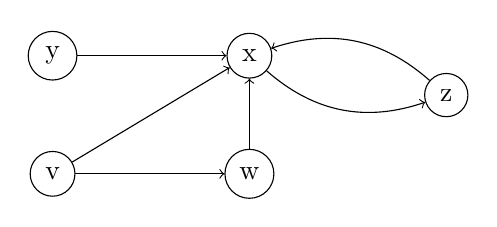
\begin{tikzpicture}
    \node[shape=circle,draw=black] (x) at (0,0) {x};
    \node[shape=circle,draw=black] (y) at (-2.5,0) {y};
    \node[shape=circle,draw=black] (z) at (2.5,-0.5) {z};
    \node[shape=circle,draw=black] (v) at (-2.5,-1.5) {v};
    \node[shape=circle,draw=black] (w) at (0,-1.5){w};
    

    \path [->] (v) edge node[left] {} (w);
    \path [->](v) edge node[left] {} (x);
    \path [->](w) edge node[left] {} (x);
    \path [->](x) edge[bend right=30] node[left] {} (z);
    \path [->](z) edge[bend right=30] node[right] {} (x);
    \path [->](y) edge node[left] {} (x);

 \end{tikzpicture}
    \end{center}
  \item Der gleiche Graph sieht ungerichtet wie folgt aus:
	          \begin{center}
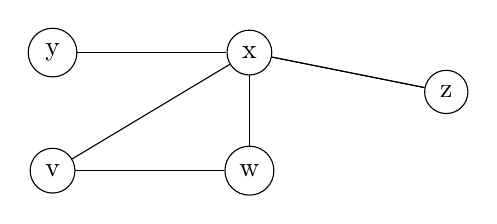
\begin{tikzpicture}
    \node[shape=circle,draw=black] (x) at (0,0) {x};
    \node[shape=circle,draw=black] (y) at (-2.5,0) {y};
    \node[shape=circle,draw=black] (z) at (2.5,-0.5) {z};
    \node[shape=circle,draw=black] (v) at (-2.5,-1.5) {v};
    \node[shape=circle,draw=black] (w) at (0,-1.5){w};


    \path [-] (v) edge node {} (w);
    \path [-](v) edge node {} (x);
    \path [-](w) edge node {} (x);
    \path [-](x) edge node {} (z);
    \path [-](z) edge node {} (x);
    \path [-](y) edge node {} (x);

 \end{tikzpicture}
    \end{center}
Wir bemerken insbesondere, dass $\{v,w\}=\{w,v\}$ im ungerichteten Graphen ist.
\end{itemize}
\end{example}
\begin{remark}
In Digraphen werden manchmal auch Kanten der Form $\{v,v\}, v \in V$ zugelassen.
\end{remark}
\begin{definition}
Sei $G=(V,E)$ ein Graph. Ein \emph{Weg} oder \emph{Pfad} von $v=v_0$ nach $w=v_r$ in $G$ ist eine Kantenfolge
\[
\pi=v_0,v_1,\ldots,v_r
\]
mit $r\ge1$ und
\begin{itemize}
	\item $(v_i, v_{i+1}) \in  E, i=0,\ldots,r-1$im Falle von Digraphen.
	\item $\{v_i,v_{i+1}\}\in E, i=0,\ldots,r-1$ im Falle von ungerichteten Graphen.
\end{itemize}
Der Weg heißt \emph{einfach}, falls
\begin{itemize}
	\item $v_0,\ldots,v_r$ paarweise verschieden sind oder
	\item $v_0,\ldots,v_r$  paarweise verschieden mit $v_0=v_r$.
\end{itemize}
Die \emph{Länge} von $\pi$ ist gegeben als $|\pi|=r$, ist also die Anzahl Knoten, die in $\pi$ durchlaufen werden.
Ein Knoten $w$ heißt von Knoten $v$ \emph{erreichbar}, falls ein Weg von $v$ nach $w$ existiert.
\end{definition}
\begin{example}
Bezogen auf Beispiel \ref{eg:graph1} ist:
\begin{itemize}
	\item $\pi_1= v,w$ ein einfacher Weg der Länge 1
	\item $\pi_2 =v,w,x$ ein einfacher Weg der Länge 2
	\item $\pi_3=v,w,x,z,x,z$ ein Weg der Länge 5
\end{itemize}
Im ungerichteten Fall ist 
\begin{itemize}
	\item $\pi_4=v,w,x,v$ ein einfacher Weg der Länge 3.
\end{itemize}
In beiden Fällen ist $z$ von $v$ erreichbar, im ungerichteten Fall gilt dies auch umgekehrt. Im gerichteten Fall ist v nicht von z erreichbar.
\end{example}
\begin{definition}
	\label{def:extendedgraph}
Sei $G=(V,E)$ ein Digraph und $v \in V$. Wir definieren:
\begin{itemize}
	\item die Menge der (direkten) \emph{Nachfahren} von v:
		\[
	post(v)=\{w \in V | (v,w) \in E\} 
		\]
	\item die Menge der (direkten) \emph{Vorfahren} von v:
		\[
		pre(v) = \{w \in  V | v \in  post(w)\} 
		\]
	\item die Menge der \emph{erreichbaren Knoten} von v:
		\[
		post^*(v)=\{w \in V | \text{ es gib einen Weg von v nach w}\} 
		\]
	\item die Menge aller Knoten die v erreichen können:
		\[
		pre^*(v)= \{w \in  V | v \in  post^*(w) \} 
		\]
	\item die Nachbarn als die Menge $post(v) \cup pre(v)$ von v
	\item und den Knotengrad $deg(v)$, welcher der Anzahl seiner Kanten entspricht.
\end{itemize}
\end{definition}
\begin{remark}
Mit den offensichtlichen Modifikationen kann die Definition \ref{def:extendedgraph} auch auf ungerichtete Graphen angewendet werden. Wir erhalten in diesem Fall für $v \in V$, dass
\begin{align*}
	post(v)&=pre(v) \\
	post^*(v) &= pre^*(v)
\end{align*}
\end{remark}
\begin{example}
Für den Digraphen aus Beispiel \ref{eg:graph1} gilt:
\begin{itemize}
	\item $post(v) = \{w,x\}$
	\item $post^*(v) = \{w,x,z\}$
	\item $pre(v)= \emptyset$
	\item $pre^*(v)= \emptyset$
	\item $deg(v)=2$
\end{itemize}
Für den ungerichteten Graphen gilt geändert:
\begin{itemize}
	\item $pre(v)=\{w,x\}$
	\item $pre^*(v)=\{w,x,y,z\}$
	\item $post^* = \{w,x,y,z\}$
\end{itemize}
\end{example}

\section{Zusammenhang}
\begin{definition}
Sei $G=(V,E)$ ein ungerichteter Graph $\emptyset \neq C \subset V$
\begin{itemize}
	\item Die Menge $C$ heißt \emph{zusammenhängend}, falls je zwei Knoten $v,w \in C , v\neq w,$ voneinander erreichbar sind, das heißt, $v \in post^*(w), w \in post^{*}(v)$. \\
Ist G ein Digraph, so heißt $C$ zusammenhängend, falls $C$ im zugrundeliegenden ungerichteten Graphen zusammenhängend ist.
\item Eine zusammenhängende Knotenmenge heißt \emph{Zusammenhangskomponente}, falls sie \emph{maximal} ist. Das bedeutet, es gibt keine weitere zusammenhängende Knotenmenge $D \subset V$ mit $C \subsetneq V$.
\item Ein Graph heißt zusammenhängend, falls $V$ zusammenhängend ist.
\end{itemize}
\end{definition}
\begin{example}
Dies ist ein unzusammenhängender Graph mit drei Zusammenhangskomponenten:
\begin{center}
\begin{tikzpicture}
    \node (A) at (0,0) {•};
    \node (B) at (0,-1) {•};
    \node (C) at (0,-2) {•};
    
    \node (D) at (2,0) {•};
    \node (E) at (1,-1) {•};

    \node (F) at (-1,0) {•};
    \node (G) at (-1,-1) {•};
    \node (H) at (-1,-2) {•};
    \node (I) at (-2,-1) {•};

    \path [-] (A) edge node {} (B);
    \path [-] (C) edge node {} (B);
    \path [-] (D) edge node {} (E);
    \path [-] (F) edge node {} (G);
    \path [-] (G) edge node {} (H);
    \path [-] (I) edge node {} (G);
\end{tikzpicture}
\end{center}
Analog hierzu ist der folgende Graph zusammenhängend:
\begin{center}
\begin{tikzpicture}
    \node (A) at (0,0) {•};
    \node (B) at (0,-1) {•};
    \node (C) at (0,-2) {•};

    \node (D) at (2,0) {•};
    \node (E) at (1,-1) {•};

    \node (F) at (-1,0) {•};
    \node (G) at (-1,-1) {•};
    \node (H) at (-1,-2) {•};
    \node (I) at (-2,-1) {•};

    \path [-] (A) edge node {} (B);
    \path [-] (C) edge node {} (B);
    \path [-] (D) edge node {} (E);
    \path [-] (F) edge node {} (G);
    \path [-] (G) edge node {} (H);
    \path [-] (I) edge node {} (G);
    
    \path [-] (B) edge node {} (G);
    \path [-] (B) edge node {} (E);
\end{tikzpicture}
\end{center}
\end{example}
Wir können beobachten, dass die Zusammenhangskomponenten eines ungerichteten Graphen die Äquivalenzklassen der Knotenmenge V unter der Äquivalenzrelation
\[
v=w \iff \{v\} \cup post^{*}(v) = \{w\} post^{*}(w) 
\]
ist. \\
Insbesondere zerfällt $G$ in paarweise disjunkte Zusammenhangskomponenten $C_1,\ldots, C_r$ mit
\begin{align*}
	V &= \bigcup_{i=1}^{r} C_i \\
	E &= \bigcup_{i=1}^{r}E_i
\end{align*}
wobei $E_i= E \cap \{X \subset C_i : |X|=2\}$.

\begin{theorem}
	\label{thm:zusammenhang}
	Sei $G=(V,E)$ ein ungerichteter Graph mit $n=|V| \ge 1$ Knoten und $m=|E|$ Kanten. Ist $G$ zusammenhängend, so folgt für die Anzahl Knoten und Kanten, dass 
\[
m \ge n-1
\]
\end{theorem}
\begin{proof}

\end{proof}
Per vollständiger Induktion:

\begin{itemize}[label=$\lozenge$, itemsep=2ex]
	\item IV \underline{n=1} \\ $m=0=n-1$
	\item IS \underline{$n \ge 3$} \\ Wähle $v \in  V$ mit:
		\[
		deg(v)= \min_{v \in V} deg(v) \eqqcolon k
		\]
		Da $G$ zusammenhängend ist, muss $k>0$ gelten. \\
		\underline{$k\ge 2$}
		\begin{align*}
		2m 
		&= 2|E| \\
		&= \sum_{w \in V} |deg{w} \\
		&\ge 2 |V| \\
		&= 2n 
		&\implies m\ge n\ge n-1
		\end{align*}
	\underline{$k=1$} \\ Sei $G'(V',E')$ derjenige Graph, der durch das Streichen von v und der zugehörigen Kante entsteht. $G'$ ist zusammenhängend, weil $G$ zusammenhängend ist. Die Induktionsannahme impliziert:
	\[
m-1=|E'| \ge |V'|-1 =(n-1)-1 = n-1 \implies m \ge n-1
	\]
\end{itemize}

\section{Zyklische Graphen}
\begin{definition}
	\label{def:zyklus}
Ein \emph{einfacher Zyklus} oder ein \emph{einfacher Kreis} in einem Graphen $G=(V,E)$ ist ein einfacher Weg $\pi =v_0,\ldots,v_r$ mit $v_0=v_r$ und $r\ge2$ (im Falle von Digraphen) oder $r \ge 3$ (im Falle von ungerichteten Graphen).
Ein \emph{Zyklus} oder \emph{Kreis} ist ein Weg, ,der sich aus einfachen Zyklen zusammensetzt.
\end{definition}

\begin{remark}
Aus der Definition \ref{def:zyklus} folgt:
\begin{itemize}
	\item Jeder einfache Zyklus ist ein Zyklus
	\item Sind $\pi_1= v_0,\ldots, v_r$, $\pi_2=w_0,\ldots,w_s$ mit $v_i=w_0=w_r$ so ist auch \\ $\pi=v_0,\ldots,v_{i-1},w_0,\ldots,w_s,v_{i+1},\ldots, v_r$ ein Zyklus
	\item Es gibt keine andere Möglichkeit um Zyklen zu generieren.
\end{itemize}
\end{remark}
\begin{example}
Der Digraph 
\begin{center}
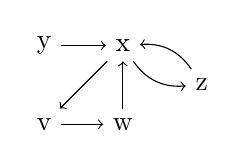
\begin{tikzpicture}
	\node (x) at (0,0) {x};
	\node (y) at (-1,0) {y};
	\node (v) at (-1,-1) {v};
	\node (w) at (0,-1) {w};
	\node (z) at (1,-0.5) {z};

	\path [->] (y) edge node {} (x);
	\path [->] (x) edge[bend right=30]  node {} (z);
	\path [->] (w) edge node {} (x);
	\path [->] (v) edge node {} (w);
	\path [->] (x) edge node {} (v);
	\path [->] (z) edge[bend right=30]  node {} (x);
\end{tikzpicture}
\end{center}
besitzt die einfachen Zyklen:
\begin{align*}
	\pi_1&=x,z,x \\
	\pi_2&=v,w,x,w
\end{align*}
und die nicht einfachen Zyklen:
\begin{align*}
	\pi_3&= x,z,x,z,x \\
	\pi_4&= v,w,x,z,x,v
\end{align*}
Der dazugehörige ungerichtete Graph:
\begin{center}
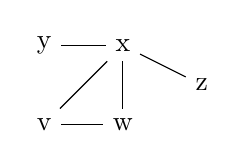
\begin{tikzpicture}
        \node (x) at (0,0) {x};
        \node (y) at (-1,0) {y};
        \node (v) at (-1,-1) {v};
        \node (w) at (0,-1) {w};
        \node (z) at (1,-0.5) {z};
        
        \path [-] (y) edge node {} (x);
        \path [-] (w) edge node {} (x);
        \path [-] (v) edge node {} (w);
        \path [-] (x) edge node {} (v);
        \path [-] (z) edge node {} (x);
\end{tikzpicture}
\end{center}
besitzt den einfachen Zyklus
\[
\pi_1= v,w,x,v
\]
Die Wege 
\begin{align*}
	\pi_2&= x,y,x \\
	\pi_3&=v,w,x,y,x,v
\end{align*}
sind keine Zyklen.
\end{example}
\subsection{Eulergraphen}
Im Folgenden betrachten wir exemplarisch das Königsberger Brückenproblem.
\begin{fluff}
Das Königsbergerbrückenproblem ist ein von Leonhard Euler gelöstes mathematisches Problem. Es handelt konkret um die Stadt Königsberg und um die Frage, ob es einen Rundweg gibt, bei dem man alle sieben Brücken der Stadt über den Pregel exakt einmal überqueren kann und wieder zum Ausgangspunkt gelangt.
\\ Euler zeigte, dass es keinen solchen Rundweg gibt.
\end{fluff}
\begin{definition}
Ein \emph{Eulerscher Rundweg} in einem Graphen $G=(V,E)$ ist ein Zyklus, der jede Kante $e \in  E$ genau einmal enthält. Im ungerichteten Fall nennen wir $G$ \emph{Eulersch}, falls der Grad jedes Knotens gerade ist. \\
Ein Digraph ist Eulersche, falls $indeg(v)= outdeg(v), v \in  V$.
\end{definition}
\begin{theorem}
	\label{thm:eulergraph}
	Ein zusammenhängender Graph $G=(V,E)$ besitzt genau dann einen Eulerschen Rundweg, falls der Graph Eulersch ist.
\end{theorem}
\begin{proof}
Hin- und Rückrichtung
\begin{itemize}
	\item \underline{$\implies$} Ein Knoten $v \in  V$ in einem Eulerschen Graph, der k-mal in einem Eulerschen Rundweg vorkommt, muss im gerichteten Fall
		\[
		indeg(v) =outdeg(v)
		\]
und im ungerichteten Fall
\[
deg(v)=2k
\]
erfüllen.
\item \underline{$\impliedby$} Sei $G$ Eulersch und $\pi=v_0,\ldots,v_r$ der längste Weg, in dem jede Kante aus $E$ höchstens einmal vorkommt.
Dies bedeutet, dass jede ausgehende Kante von $v_r$ im Weg enthalten sein muss (sonst wäre es nicht der längste Weg).
Die Bedingung an den Knotengrad impliziert: $v_0=v_r$.
\paragraph{Annahme:}
\begin{itemize}
	\item Digraphen: Es gibt eine Kante $e=(w_1,w_2) \in  E $ mit \\$e \neq (v_i, v_{i+1}, i=0,\ldots,r-1$
	\item ungerichtete Graphen: Es gibt eine Kante $e=\{w_1,w_2\} \in  E$ mit $e \neq \{v_i,v_{i+1}\}, i=0,\ldots,r-1$.
\end{itemize}
\underline{Fall 1:} $w_1 \text{ oder }w_2$ sind in $\pi$ enthalten. \\
Ohne Beschränkung der Allgemeinheit: $v_r=w_1$
\[
\implies \tilde{\pi} =v_0,\ldots,v_r,w_2
\]
Dies ist ein Widerspruch zur Annahme, da $\pi$ nun nicht mehr der längste Weg ist. \\
\underline{Fall 2:} $w_1$ und $w_2$ sind beide nicht in $\pi$ enthalten.
Da $G$ zusammenhängend ist, gibt es einen Weg von $v_0$ nach $w_1$. Entlang dieses Weges muss es eine Kante geben, die einen Knoten in $\pi$ und einen nicht in $\pi$ hat. \\
Analog zum ersten Fall führt dies zum Widerspruch.
\end{itemize}
\end{proof}
Wir beachten: Satz \ref{thm:eulergraph} ist die Antwort auf das Königsberger Brückenproblem. Demnach gibt es keinen solchen Weg und es ist nicht mögliche einen Euler-Weg zu finden.

\section{Bäume}
\begin{definition}
Ein Graph $G$ heißt \emph{azyklisch} oder \emph{zyklenfrei}, falls es keine Zyklen in $G$ gibt. Ein ungerichteter, azyklischer und zusammenhängender Graph ist ein \emph{Baum}
\end{definition}
\begin{example}
Ein azyklischer Graph kann wie folgt aussehen:
\begin{center}
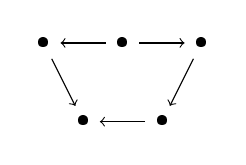
\begin{tikzpicture}
	\node (1) at (0,0) {•};
	\node (2) at (1,0) {•};
	\node (3) at (-1,0) {•};
	\node (4) at (0.5,-1) {•};
	\node (5) at (-0.5, -1) {•};


	\path [->] (1) edge node {} (2);
	\path [->] (1) edge node {} (3);
	\path [->] (2) edge node {} (4);
	\path [->] (4) edge node {} (5);
	\path [->] (3) edge node {} (5);	
\end{tikzpicture}
\end{center}
Sollte dieser ungerichtet sein könnte er so aussehen:
\begin{center}
\begin{tikzpicture}
	\node (1) at (0,0) {•};
	\node (2) at (2,0) {•};
	\node (3) at (1,-1) {•};
	\node (4) at (3,-1) {•};
	
	\node (5) at (-2,0) {•};
	\node (6) at (-1,-1) {•};
	\node (7) at (-3,-1) {•};

	\path [-] (1) edge node {} (2);
	\path [-] (1) edge node {} (5);
	\path [-] (2) edge node {} (3);
	\path [-] (3) edge node {} (4);
	\path [-] (5) edge node {} (6);
	\path [-] (5) edge node {} (7);
\end{tikzpicture}
\end{center}
Dieser Graph ist sogar zusammenhängend.
\end{example}
\begin{theorem}
Sei $G=(V,E)$ ein ungerichteter Graph mit $n=|V|$ knoten. Dann sind die folgenden Aussagen äquivalent.
\begin{enumerate}
	\item G ist ein Baum
	\item G hat n-1 Kanten und ist zusammenhängend
	\item G hat n-1 Kanten und ist azyklisch
	\item G ist azyklisch und das Hinzufügen einer beliebigen, noch nicht vorhandenen Kante erzeugt einen Zyklus.
	\item G ist zusammenhängend und das Entfernen einer beliebigen Kante macht G unzusammenhängend.
	\item Jedes Paar verschiedener Knoten in G ist durch genau einen einfachen Weg miteinander verbunden.
\end{enumerate}
\end{theorem}
\begin{proof}
Wir zeigen nicht jede Äquivalenz einzeln, sondern folgern aus anderen Aussagen.\begin{itemize}
	\item \underline{$a \implies f$} Falls es für ein gegebenes Paar $v,w \in  V$, verschiedene Wege gäbe, so würde die Vereinigung dieser beiden Wege einen Zyklus beinhalten (Widerspruch zu azyklisch in Baum).
	\item \underline{$f \implies e$} "zusammenhängend" folgt per Definition.
		Falls wir eine beliebige Kante entfernen, so sind die beiden Endpunkte nicht mehr voneinander erreichbar ( $\implies$ G wird unzusammenhängend).
	\item \underline{$e \implies d$} G ist azyklisch, da wir sonst eine (ausgewählte) Kante entfernen könnten, so dass g immer noch zusammenhängend wäre. Seien $v,w \in  V, w \neq v$, dann gibt es einen Weg von v nach w. 
	Hinzufügen der Kante $\{v,w\}$ macht diesen Weg zum Zyklus.
\item \underline{$d \implies c$} Wir zeigen per Induktion über $m= |E|$, dass für einen azyklischen, ungerichteten Graph
	\begin{equation}
	\label{eqn:keinplan}
		n=m+p
	\end{equation}
	gilt, wobei p die Anzahl Zusammenhangskomponenten ist.
	\begin{itemize}[label=$\lozenge$, itemsep=2ex]
		\item IV \underline{$m=0$} trivial
		\item IS \underline{$m \to m+1$} Beim Hinzufügen einer Kante muss eine Zusammenhangskomponente verschwinden, da sonst ein Zyklus entstehen würde. \\
	Da das Hinzufügen einer beliebigen neuen Kante einen Zyklus entstehen lässt, muss $p=1$ gelten.
	\[
	\implies |E|=m=n-1
	\]
	\end{itemize}
\item \underline{$c \implies b$} Folgt aus \eqref{eqn:keinplan}
\item \underline{$b \implies a$} Zu zeigen: $G$ ist azyklisch. \\
	Angenommen $G$ hat $k$ verschiedene einfache Zyklen. Dann können wir $G$ durch entfernen von $k$ Kanten zu einem azyklischen Graphen machen. \eqref{eqn:keinplan} ist andwendbar, un impliziert, dass 
	\begin{align*}
		n &= (m-k)+1 \\
		m+1 &= (m-k)+1 		    &\implies k=0
	\end{align*}
	d.h. $G$ keine Zyklen.
\end{itemize}
\end{proof}
\begin{remark}
Fixieren wir in einem Baum $G=(V,E)$ einen Wurzelknoten, so wird automatisch eine Richtung in den Kanten festgelegt. Für $v \in V$ heißt $pre(v), |pre(v)|=1$ der \emph{Elternteil} und $post(v)$ die \emph{Kinder}.
\end{remark}

\section{Implementierung von Graphen}
\begin{definition}
Ein Graph $G=(V,E)$ mit $V=\{1,\ldots,n\}$ kann durch einen \emph{Adjazenzmatrix} oder \emph{Nachbarschftsmatrix}
\[
A = [a_{i,j} ]_{i,j=1}^{n} \in  \R^{n,n}
\]
mit
\begin{center}
$a_{i,j} = \begin{cases}
	1 &, \text{ falls } (i,j) \in  E, \text{ bzw. falls } \{i,j\} \in E \\
	0 &, \text{ sonst}
\end{cases}$
\end{center}
dargestellt werden.
\end{definition}
\begin{example}
Der gerichtete Graph
\begin{center}
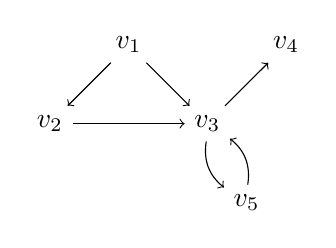
\begin{tikzpicture}
	\node (v1) at (0,0) {$v_1$};
	\node (v2) at (-1,-1) {$v_2$};
	\node (v3) at (1,-1) {$v_3$};
	\node (v4) at (2,0) {$v_4$};
	\node (v5) at (1.5,-2) {$v_5$};

	\path [->] (v1) edge node {} (v2);
	\path [->] (v1) edge node {} (v3);
	\path [->] (v2) edge node {} (v3);
	\path [->] (v3) edge node {} (v4);
	\path [->] (v3) edge[bend right=30] node {} (v5);
	\path [->] (v5) edge[bend right=30] node {} (v3);
\end{tikzpicture}
\end{center}
besitzt die Adjazenzmatrix
\[
A= \begin{bmatrix}
	0 & 1 & 1 & 0 & 0 \\
	0 & 0 & 1 & 0 & 0 \\
	0 & 0 & 0 & 1 & 1 \\
	0 & 0 & 0 & 0 & 0 \\
	0 & 0 & 1 & 0 & 0
\end{bmatrix}
\]
und falls der Graph als ungerichteter Graph aufgefasst wird:
\[
A = \begin{bmatrix}
	0&1&1&0&0\\
	1&0&1&0&0\\
	1&1&0&1&1\\
	0&0&1&0&0\\
	0&0&1&0&0
\end{bmatrix}
\]
\end{example}

\begin{remark}
Bei ungerichteten Graphen ist die Adjazenzmatrix \underline{immer} symmetrisch.\\
Der Speicherbedarf einer Adjazenzmatrix ist $|V|^2$, unabhängig von $|E|$. Für größere Graphen ist dies ineffizient. 
Wir werden beim Behandeln von dünnbesetzten Matrizen ein alternatives Speicherformat kennenlernen. \\
Zum Abschluss bemerken wir, dass sich viele graphentheoretische Konzepte mir Hilfe der Adjazenzmatrix in die Sprach der linearen Algebra übersetzten lässt.
\end{remark}


\addchap{Algorithmen auf Graphen}
\section{Graphendurchmusterung}
Graphen müssen häufig durchmustert, d.h systematisch durchsucht, werden. Im Folgenden werden wir die "Tiefensuche" und die "Breitensuche" betrachten, welche sich beide auf den folgenden Algorithmus zurückführen lassen:\\

\begin{algorithm}[H]
\label{alg:algorithmische_suche}
\caption{Algorithmische Suche}
\KwData{Graph $G=(V,E)$, Startknoten $s \in V$}
\KwResult{Zusammenhängender, azyklischer Graph $G'(R,T)$ mit $R=\{s\} \cup post^{*}(s)$ und $T \subset E$}
\begin{itemize}
	\item $R=\{s\}$
	\item $Q= \{s\}$
	\item $T= \emptyset$
	\item (a) \If{$Q= \emptyset$}{stop}
		\Else{Wähle $v \in  Q \subset R$}
	\item Wähle $w \in  V \setminus R \cap post(v)$
		\If{ kein solches $w$ exisitert}{setze $Q= Q \setminus \{v\}$ und gehe zu (a)}
	\item $R=R \cup \{w\}$
	\item $Q=Q \cup \{w\} $
	\item $T= T \cup \{e\} $ mit $e=(v,w)$ oder $e=\{v,w\} $
	\item Gehe zu (a)
\end{itemize}
\end{algorithm}
Je nachdem wie $v \in Q$ gewählt wird, bezeichnen wir den Suchalgorithmus unterschiedlich:
\begin{definition}
Bei der \emph{Tiefensuche} oder \emph{Depth-First-Search} (DFS) wird derjenige Knoten in $v \in  Q$ ausgewählt, der zuletzt zu $Q$ hinzugefügt wurde. Bei der \emph{Breitensuche} oder \emph{Breadth-First-Search} (BSF) wird derjenige Knoten $v \in  Q$ ausgewählt, der zuerst zu Q hinzugefügt wurde.
\end{definition}
\begin{theorem}
Algorithmus \ref{alg:algorithmische_suche} liefert einen zusammenhängenden, azyklischen Graphen $G'(R,T)$, mit $R=\{s\}\cup post^{*}(s)$ und $T \subset E$.
\end{theorem}
\begin{proof}
Per Konstruktion ist $(R,T)$ zu jedem Zeitpunkt im Algorithmus zusammenhängend.\\
$(R,T)$ ist außerdem zu jedem Zeitpunkt azyklisch, denn per Konstruktion gilt $Q \subset R$ und $e$ verbindet jeweils $v \in  Q \subset R$ mit $w \in  V \setminus R$. Wir müssen also zeigen: $R = \{s\} \cup post^{*}(v)$ ($T \subset E$ ist klar). \\
\underline{Annahme:} Nach Ende des Algorithmus gibt es $w \in  V \setminus R$ von $s$ erreichbar. Dann gibt es einen Weg \[
\pi = s,v_1,\ldots,v_r, w
\]
und darin eine Kante $e=(x,y) \in E$ bzw. $e >\{x,y\} \in E$, mit $x \in R$ und $y \not\in R$, $x,y \in \{s,v_1,\ldots,v_r,w\} $.
Da $x \in  R$, muss zu einem gewissen Zeitpunkt im Algorithmus auch $x \in  Q$ gelten. Der Algorithmus terminiert, aber nur, falls $x$ aus $Q$ entfernt wurde, was nur geschieht, wenn $y \not\in V \setminus R \cap post(x)$, also falls $e \not\in E$ ist. \\
Dies ist ein Widerspruch zu unserer Annahme.
\end{proof}
\begin{example}
Betrachte 
\begin{center}
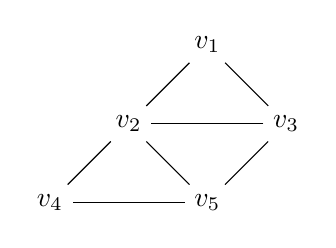
\begin{tikzpicture}
 \node (v1) at (0,0) {$v_1$};
 \node (v2) at (-1,-1) {$v_2$};
 \node (v3) at (1,-1) {$v_3$};
 \node (v4) at (-2,-2) {$v_4$};
 \node (v5) at (0,-2) {$v_5$};

 \path [-] (v1) edge node {} (v2);
 \path [-] (v1) edge node {} (v3);
 \path [-] (v3) edge node {} (v2);
 \path [-] (v4) edge node {} (v2);
 \path [-] (v5) edge node {} (v2);
 \path [-] (v5) edge node {} (v4);
 \path [-] (v3) edge node {} (v5);
\end{tikzpicture}
\end{center}
$s =\{v_1\}$. Bei der Tiefensuche entsteht folgender Baum:
\begin{center}
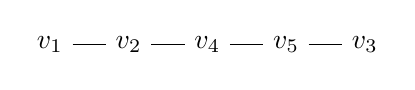
\begin{tikzpicture}
\node (v1) at (0,0) {$v_1$};
\node (v2) at (1,0) {$v_2$};
\node (v3) at (4,0) {$v_3$};
\node (v4) at (2,0) {$v_4$};
\node (v5) at (3,0) {$v_5$};

\path [-] (v1) edge node {} (v2);
\path [-] (v2) edge node {} (v4);
\path [-] (v4) edge node {} (v5);
\path [-] (v5) edge node {} (v3);
\end{tikzpicture}
\end{center}
Die Breitensuche hingegen ergibt:
\begin{center}
\begin{tikzpicture}
\node (v1) at (0,0) {$v_1$};
\node (v2) at (-1,-1) {$v_2$};
\node (v3) at (1,-1) {$v_3$};
\node (v4) at (-2,-2) {$v_4$};
\node (v5) at (0,-2) {$v_5$};

\path [-] (v1) edge node {} (v2);
\path [-] (v1) edge node {} (v3);
\path [-] (v2) edge node {} (v4);
\path [-] (v2) edge node {} (v5);	
\end{tikzpicture}
\end{center}
\end{example}
\begin{remark}
Ist $G$ ein ungerichteter Graph, so ist das Resultat $G'$ von Algorithmus \ref{alg:algorithmische_suche} ein Baum mit Wurzel $s$, der \emph{Spannbaum}
\end{remark}
\begin{theorem}
	\label{thm:algorithmische_suche}
	Die Ausführung von "wähle $v \in Q$" und "wähle $w \in  V \setminus R \cap post(v)$" sei in $\mathcal{O}(1)$ durchführbar. Dann besitzt Algorithmus \ref{alg:algorithmische_suche} den linearen Aufwand $\mathcal{O}(|V|+|E|)$.
\end{theorem}
\begin{proof}
"wähle $v \in Q$" wird maximal $(|post(v)|+1)$ mal aufgerufen. \\
"wähle $w \in V \setminus R \cap post(v)$" wird für jede Kante maximal ein mal aufgerufen. \\
Daraus folgt direkt die Behauptung.
\end{proof}
Wir hatten gezeigt, (Satz \ref{thm:zusammenhang}), dass $|V|-1 \le |E|$, d.h, es gilt $\mathcal{O}(|V|+|E|)$ kann nach oben beschränkt werden durch $\mathcal{O}(2|E|)$.
\paragraph{Beobachtung:} Die Breitensuche beschreibt einen "kürzesten" Weg von Startknoten zu jedem anderen Knoten.

\begin{theorem}
	Sie $G=(V,E)$ ein ungerichteter Graph, $s,v \in V$ und \\ $dist_G(s,v)= \min \{|\pi| : \pi = s,u_1,\ldots,u_r,v \text{ ein Weg in G}\}$ mit $dist_G(s,v) = \infty $, falls es keinen Weg von $s$ nach $v$ gibt. 
Dann enthält der durch die Breitensuche erzeugte Graph $G'=(R,T)$ zum Startknoten $s \in V$ einen kürzesten Weg zu jedem Knoten $v \in  post^{*}(s)$.Dies bedeutet, es gib einen einfachen Weg $\pi=s,u_1,\ldots,u_r,v$ in $G'$ mit $|\pi|= dist_{G'}(s,v)= dist_G(s,v)$ minimal.
\end{theorem}
\begin{proof}
Wir bemerken zuerst, dass $G'$ azyklisch ist und somit $\pi$ in $G'$ eindeutig bestimmt ist.
Modifiziere Algorithmus \ref{alg:algorithmische_suche} nun wie folgt:
\begin{itemize}
	\item In 1: l(s)=0
	\item In 4: l(w) = l(v)+1
\end{itemize}
Dies bedeutet, zu jedem Zeitpunkt im Algorithmus gilt:
\[
l(v)=dist_{(R,T)} (s,v) , v \in R
\]
Insbesondere gibt es für kein in 2 ausgewähltes $v \in  Q$ ein $w \in R$ mit:
\begin{equation}
	\label{eqn:dist1}
l(w)> l(v)+1
\end{equation}
\underline{Zu Zeigen:} $dist_{R,T} (s,v) = dist_{G'} (s,v) = dist_G (s,v)$ \\
\underline{Annahme:} Nach Abbruch des Algorithmus gibt es ein $w \in V$ mit 
\begin{equation}
\label{eqn:dist2}
dist_G(s,w) < dist_{G'} (s,w)
\end{equation}
Falls es mehr als ein solches $w$  gibt , wähle dasjenige mit den kleinsten Abstand 
$dist_G(s,w)$.\\
Sei $\pi=s,u_1,\ldots,u_r,v,w \implies dist_G(s,v) = dist_{G'} (s,v)$ , da sonst v ein Knoten mit kleineren Abstand wäre, der \eqref{eqn:dist2} erfüllt.
\begin{align*}
	\implies l(w) &= dist_{G'}(s,w) \\
		      &> dist_G(s,w) \\
		      &= dist_G (s,v) +1 \\
		      &= dist_{G'} (s,v)+1 \\
		      &=l(v) +1
\end{align*}
Dies ist ein Widerspruch zu \eqref{eqn:dist1}.
\end{proof}
\begin{remark}
Die Breitensuche berechnet also die Wege aller Knoten zur Wurzel in $\mathcal{O}(|V|+|E|)$ .
\end{remark}

\section{Starker Zusammenhang}
\begin{definition}
Ein Digraph heißt \emph{stark zusammenhängend}, falls für jedes Knotenpaar $v,w \in  V$ , $v \neq w$ , sowohl $v \in  post^{*}(w)$ , als auch $w \in post^{*}(w)$ gilt.
Es gibt also einen Weg von $v$  nach $w$  und umgekehrt. \\ 
Die \emph{starken Zusammenhangskomponenten} sind die maximalen stark zusammenhängenden Teilgraphen.
\end{definition}
\begin{example}
	Der Graph:
\begin{center}
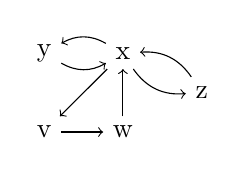
\begin{tikzpicture}

	\node (x) at (0,0) {x};
	\node (y) at (-1,0) {y};
	\node (z) at (1,-0.5) {z};
	\node (v) at (-1,-1) {v};
	\node (w) at (0,-1) {w};

	\path [->] (x) edge[bend right=30] node {} (y);
	\path [->] (y) edge[bend right=30] node {} (x);
	\path [->] (x) edge[bend right=30] node {} (z);
	\path [->] (z) edge[bend right=30] node {} (x);
	\path [->] (w) edge node {} (x);
	\path [->] (v) edge node {} (w);
	\path [->] (x) edge node {} (v);
\end{tikzpicture}
\end{center}
ist stark zusammenhängend.
\begin{center}
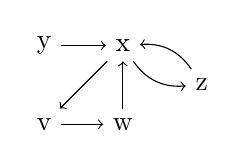
\begin{tikzpicture}

        \node (x) at (0,0) {x};
        \node (y) at (-1,0) {y};
        \node (z) at (1,-0.5) {z};
        \node (v) at (-1,-1) {v};
        \node (w) at (0,-1) {w};

        \path [->] (y) edge node {} (x);
        \path [->] (x) edge[bend right=30] node {} (z);
        \path [->] (z) edge[bend right=30] node {} (x);
        \path [->] (w) edge node {} (x);
        \path [->] (v) edge node {} (w);
        \path [->] (x) edge node {} (v);
\end{tikzpicture}
\end{center}
Dieser Graph, wo der Weg von x nach y entfernt wurde, ist nicht stark zusammenhängend. Die starken Zusammenhangskomponenten sind y und der restliche Graph $G'$.
\end{example}
Im folgenden konstruieren wir einen Algorithmus zur Bestimmung solcher starker Zusammenhangskomponenten.

\begin{algorithm}[H]
\label{alg:starker_zusammenhang}
\caption{Bestimmung starker Zusammenhangskomponenten}
\KwData{Digraph $G=(V,E)$}
\KwResult{Abbildung $comp \colon V \to \N $, welche die Zugehörigkeit zu einer starken Zusammenhangskomponente signalisiert.} 
\begin{itemize}
	\item $R = \emptyset$
	\item $N=0$ 
	\item \For{$v \in V$}{ \If {$v \not\in R$ }{FirstVisit(v)}}
	\item $R = \emptyset$
	\item $K=0$
	\item \For{$j \gets |V|$ \KwTo 1}{{\If{ $\psi^{-1}(j) \not\in R$}{$K=K+1$ \\
		SecondVisit($\psi^{-1}(j)$) } }}	
\end{itemize}
\SetKwFunction{FirstVisit}{FirstVisit}
\SetKwFunction{SecondVisit}{SecondVisit}
 \SetKwProg{Fn}{Function}{}{\KwRet}
\Fn{\FirstVisit{v}{
\begin{itemize}
	\item $R = R \cup \{v\} $ 
	\item \For{$w \in V \setminus R$, $(v,w) \in E$}{FirstVisit(w)}
	\item $N=N+1$ 
	\item $\psi(v)=N$ 
	\item $\psi^{-1}(N)=V$ 
\end{itemize}
}}

\Fn{\SecondVisit{v}{
\begin{itemize}
	\item $R = R \cup \{w\} $ 
	\item \For{$w \in V \setminus R$, $(w,v) \in E$}{SecondVisit(w)}
	\item $comp(v)=K$ 
\end{itemize}
}}

\end{algorithm}

\begin{example}
Wir betrachten den Graph:
\begin{center}
\begin{tikzpicture}

\end{tikzpicture}
\end{center}
Der Startknoten $v_1$ für FirstVisit ergibt die Besuchsreihenfolge: $v_1,v_7,v_2,v_4,v_5$.
Die Tiefensuche mittels FirstVisit bricht für $v_3$ und $v_6$ direkt ab.
Wir erhalten:
\begin{align*}
	\psi(v_2)&=1 & \psi(v_7) &=4 & \psi(v_6)=7 \\
	\psi(v_5)&=2 & \psi(v_1)&=5 \\
	\psi(v_4)&=3 & \psi(v_3)&=6
\end{align*}
SecondVisit für $v_6= \psi^{-1}(7) $ bricht sofort ab $\implies comp(v_6)=1$ \\
SecondVisit für $v_3=\psi^{-1}(6) $ bricht sofort ab $\implies comp(v_3)=2$\\
SecondVisit für $v_1=\psi^{-1}(5)$ ergibt die Besuchsreihenfolge: $v_2,v_7 \implies comp(v_1)=3, v \in \{v_1,v_2,v_7\} $ \\
SecondVisit für $v_4= \psi^{-1}(3)$ ergibt die Besuchsreihenfolge: $v_5 \implies comp(v_4)=4$. 
Demnach ergibt sich:
\[
\{v_6\} , \{v_3\} , \{v_1,v_2,v_7\} , \{v_4,v_5\} 
\]
\end{example}
\begin{theorem}
	Algorithmus \ref{alg:starker_zusammenhang} identifiziert die starken Zusammenhangskomponenten eines Digraphen $G=(V,E)$ in linearem Aufwand $\mathcal{O}(|V|+|E|)$
\end{theorem}
\begin{proof}
	 Aufwand: Analog zur Tiefensuche (Satz \ref{thm:algorithmische_suche})
\begin{itemize}
	\item \underline{Gleiche starke Zusammenhangskomponente $\\implies $ gleicher comp-Wert} \\
Seien $v,w \in V$ Knoten in der gleichen , starken Zusammenhangskomponente \\
\begin{itemize}
	\item $\implies $ Es gibt einen Weg von $v$ nach $w$ und umgekehrt.
	\item $\implies $ SecondVisit weist $comp(v)=comp(w)$ zu
\end{itemize}
\item \underline{Gleicher comp-Wert $\implies $ Gleiche starke Zusammenhangskomponente} \\
Seien $v,w \in V$ mit $comp(v)=comp(w)$. Definiere $r(v)$ ist derjenige von $v$  erreichbare Knoten, der den höchsten $\psi$-Wert hat. \\
\emph{Beobachte:}
\begin{itemize}
	\item $comp(v)=comp(w) \implies v \text{ und } w$  sind im gleichen, von SecondVisist erzeugten Subbaum.
	$\implies r(v)=r(w) \eqqcolon r$ (d.h r ist von $v,w$ erreichbar)
\item $\psi(r)>\psi(v) \implies v$ wurde in FirstVisit vor $r$ nummeriert. $\implies $ Der von FirstVisit erzeugte Baum hat einen Weg von $r$ nach $v$ , d.h $v$ ist von $r$ erreichbar.
\item Analog: $w$ ist von $r$ erreichbar. $\implies v$ ist über $r$ von $w$  aus erreichbar und umgekehrt. 
\end{itemize}
\end{itemize}
\end{proof}
\begin{definition}
	Sei $G=(V,E)$  ein Digraph. Zieht man die starken Zusammenhangskomponenten zu einem Knoten zusammen, entsteht ein \emph{kondensierter Graph}. \\
Eine \emph{Nummerierung} $v=\{v_1,\ldots,v_n\}$ der Knoten heißt \emph{topologische Ordnung}, falls $(v_i, v_j) \in  E$ nur, wenn $i<j$.
\end{definition}
\begin{lemma}
	\label{lem:topo_ordnung}
Der Digraph $G=(V,E)$  besitzt eine topologische Ordnung genau dann, wenn er azyklisch ist.
\end{lemma}
\begin{proof}
Übung
\end{proof}
\begin{theorem}
	Zu jedem Digraphen $G=(V,E)$  bestimmt Algorithmus \ref{alg:starker_zusammenhang} eine topologische Ordnung in linearem Aufwand $\mathcal{O}(|V|+|E|)$.
	Gibt es eine solche Ordnung nicht, so sagt uns das der Algorithmus ebenfalls in linearem Aufwand.
\end{theorem}
\begin{proof}
Seien $V_i, V_j \subset V$ die (disjunkten) Knotenmengen zweier stabiler Zusammenhangskomponenten mit $comp(v_i)=i, comp(v_j)=j$ für $v_i \in  V_i, v_j \in  V_j$. \\
Ohne Beschränkung der Allgemeinheit: $i<j$\\
\underline{Annahme:} Es gibt eine Kante $e=(v_j,v_i)$ mit $v_j \in  V_j, v_i \in  V_i$ .
\emph{Beobacht:} In SecondVisit werden alle Knoten in $V_i$ vor derjenigen in $V_j$ zu $R$ hinzugefügt. $\implies $ 
\begin{itemize}
	\item Beim Überprüfen von $e=(v_j,v_i)$ in SecondVisit gilt: $v_i \in R, v_j \not\in R$ 
	\item $v_j$  wird zu $R$ hinzugefügt, bevor $K$ erhöht wird.
	\item $comp(v_i)=comp(v_j)$ 
\end{itemize}
Dies ist ein Widerspruch. \\
$\implies $ Algorithmus \ref{alg:starker_zusammenhang} erzeugt eine topologische Ordnung, falls diese existiert. \\
Aus Lemma \ref{lem:topo_ordnung} folgt: \\
Es gibt genau dann eine topologische Ordnung auf $G$, falls $G$ azyklisch ist.\\
$\iff $ alle starken Zusammenhangskomponenten sind eindeutig. \\
$\iff $ Am Ende des Algorithmus ist $K=|V|$ 
\end{proof}
\begin{remark}
Der Beweis zeigt, dass Algorithmus \ref{alg:starker_zusammenhang} auch benutzt werden kann, um in linearer Zeit zu überprüfen, ob ein Graph Zyklen hat.
\end{remark}

\input{chapters/sections-alma1/kürzeste-wege}
\section{Netzwerkflussprobleme}
\begin{example}
Ausgehend von einer Bananenplantage s sollen alle geernteten Bananen zum Lagerhaus t transportiert werden. Für den Transport stehen Straßen mit $r_1,\ldots,r_p$ $\frac{kg}{n}$ Transportkapazität zu den Seehäfen $A_1,\ldots,A_p$ zu Verfügung. Von den Zielhäfen $B_1,\ldots,B_q$ stehen Transportkapazitäten von $d_1,\ldots,d_q$ $\frac{kg}{n}$ zum Supermarkt t bereit.
Die Transportkapazität zwischen den Seehäfen werden mit $c(A_i,A_j), 1\le i\le p, 1\le j \le p$ bezeichnet.
\paragraph{Fragen:}
\begin{itemize}
	\item Ist es mögliche, alle Transportkapazitäten auszuschöpfen?
	\item Falls nein, was ist die maximal mögliche Transportkapazität?
	\item Wie sollen die Bananenladungen aufgeteilt werden?
\end{itemize}
Konstruiere einen gewichteten Digraph $G=(V,E,w)$ mit
\begin{itemize}
	\item $V=\{s, A_1,\ldots,A_p, B_1,\ldots,q,t\} $ 
	\item $E= \{(s,A_i), (A_i,B_j), (B_j,t) ; 1\le i\le p, 1\le j\le p\} $ 
	\item $w(e)= \begin{cases}
			r_i &, e=(s,A_i) \\
			c(A_i,B_j) &, e(A_i,B_j) \\
			d_i &, e(B_i,t)
	\end{cases}$ 
\end{itemize}

\begin{center}
\begin{tikzpicture}


	%Netzwerk einfügen


\end{tikzpicture}
\end{center}
\end{example}
\begin{definition}
Ein \emph{Netzwerk} ist ein Tupel $N=(V,E,c,s,t)$  bestehend aus
\begin{itemize}
	\item einem gewichteten Digraphen $G=(V,E,c)$
	\item einer \emph{Kapazitätsfunktion} $c \colon E \to R_{\ge 0}$
	\item einer Quelle $s \in V$ mit $pre(s)= \emptyset$ 
	\item einer Senke $t \in V$ mit $post(t)=\emptyset$ 
\end{itemize}
Ein Fluss $f \colon E \to R_{\ge 0}$ ist eine Funktion, die folgende Bedingungen erfüllt:
\begin{enumerate}
	\item \emph{Kapazitätsbedingung:}
		\[
		f(v,w) \le c(v,w)
		\]
	\item \emph{Kirchhoffsches Gesetz:}
		\[
		\sum_{u \in pre(v)} f(u,v) = \sum_{w \in  post(v)} f(v,w)
		\]
für alle $v \in V \setminus \{s,t\} $ .
\end{enumerate}
Der \emph{Wert} des Flusses ist:
\[
flow(f) = \sum_{w \in post(s)}f(s,w)
\]
Der \emph{maximale FLuss} von N wird bezeichnet als:
\[
MaxFlow(N) = \max \{flow(f) \text{ ist Fluss für N}\} 
\]
Eine Flussfunktion $f$ wird \emph{optimal} genannt, falls 
\[
flow(f)=MaxFlow(N)
\]
ist. \\
Ein \emph{Schnitt} für N ist eine Knotenmenge $S \subset V$ mit $s \in S, t \not\in S$. \\
Die \emph{Kapazität} eines Schnittes ist gegeben durch:
\[
cap(S)= \sum_{v \in S \\ w \in post(v) \setminus S}c(v,w)
\]
Die minimale Schnittkapazität von N ist:
\[
MinCut(N)= \min \{cap(S) | \text{ S ist Schnitt für N}\} 
\]
\end{definition}
\begin{lemma}
	Sei S ein Schnitt für $N=(V,E,c,s,t)$. Dann gilt für jeden Fluss f, dass
	\begin{align*}
		flow(f) &= \sum_{w \in post(v) \setminus S} f(v,w) - \sum_{u \in  pre(v)} f(u,v) \\
		flow(f) &\le cap(S)
	\end{align*}
\end{lemma}
\begin{proof}
Rechne:
\begin{align*}
	flow(f) &= \sum_{w \in post(s)} f(s,w) \\
		&= \sum_{v \in S}\left( \sum_{w \in post(v)}f(v,w)- \sum_{u \in pre(v)}f(u,v) \right)\\
		&=\sum_{w \in post(v)}f(v,w) - \sum_{u \in pre(v) \setminus S}f(u,v)
\end{align*}
Für die nächste Behauptung können wir ebenfalls nachrechnen:
\begin{align*}
	flow(f) &= \sum_{w \in post(v) \setminus S} f(v,w) - \sum_{u \in pre(v) \setminus S}f(u,v) \\
		&\le \sum_{w \in post(v) \setminus S}c(v,w) \\
		&=cap(S)
\end{align*}
\end{proof}
\begin{theorem}[Max-FLow-Min-Cut Theorem]
\label{thm:min-cut}
Sei $N=(V,E,c,s,t)$ ein Netzwerk, dann gilt:
\[
MaxFlow(N)=MinCut(N)
\]
\end{theorem}
\begin{proof}
\underline{Zu zeigen:} Es gibt einen Schnitt für den die Gleichheit gilt. \\
\underline{Idee:} Gegeben sei ein Fluss f mit flow(f)=MaxFlow(N), konsturiere einen Schnitt $S$ mit flow(f)=cap(S). \\
\begin{algorithm}[H]
\label{alg:beweis-max-min}
\KwData{Netzwerk $N$, Fluss $f$ mit $flow(f)=MaxFlow(N)$.}
\KwResult{S mit $flow(f)=cap(S)$}
\begin{itemize}
	\item $S=\{s\}$ 
	\item \While{$x \in S, y \in V \setminus S$ existieren mit $\begin{cases}
				f(x,y) < c(x,y) &, \text{ falls } (x,y) \in E \\
				0 < f(y,x) &, \text{ falls } (y,x) \in E
	\end{cases}$ \\ dann }{$S=S \cup \{y\}$}
\end{itemize}
\end{algorithm}
\underline{Behauptung} Das Resultat $S$ des Algorithmus ist ein Schnitt von $N$
\begin{proof}
Zu Zeigen: $t \not\in S$ \\
\underline{Angenommen:}  $t \in S, v_r=t$ \\
$\implies$ Es gibt $v_{r-1} \in S$ mit $f(v_{r-1},v_r) < c(v_{r-1},v_r)$. \\
Iterativ: Es gibt einen ungerichteten Weg $\pi$ mit $v_0=s, v_r=t$\\
Definiere für $i=0,\ldots,r-1$:
\[
\varepsilon_i = \begin{cases}
	c(e)-f(e) &, \text{ falls } e=(v_i,v_{i+1}) \in E , e^{-1}=(v_{i+1}, v_i) \not\in E \\
	f(e^{-1}) &, \text{ falls } e \not\in E , e^{-1} \in E \\
	\max \{c(e)-f(e), f(e^{-1})\} &, \text{ falls } e \in E , e^{-1} \in E
\end{cases}
\]
Beobachte: $\varepsilon_i > 0$
\begin{equation}
	\label{eqn:epsilon}
\varepsilon = \min_{ß\le i \le r-1} \varepsilon_i > 0
\end{equation}
\underline{Zeige:} Es gib einen Fluss $f^{*}$ in $N$  mit $flow(f^{*}) = flow(f)+\varepsilon$ \\
\underline{Konstruiere:}
\[
f^{*}(e)= \begin{cases}
	f(e)+\varepsilon &, \text{ falls } e=(v_i, v_{i+1} \in E, e^{-1}\not\in E \\
	f(e)-\varepsilon &, \text{ falls } e = (v_{i+1}, v_i) \in E, e^{-1}\not\in E \\
	f(e)+\varepsilon &, \text{ falls } e=(v_i, v_{i+1}), e^{-1} \in E \text{ und } c(e)-f(e) > f(e^{-1}) \\
	f(e)-\varepsilon &, \text{ falls } e=(v_{i+1}, v_i), e^{-1} \in E \text{ und } c(e)-f(e) \le f(e^{-1}) \\
	f(e) &, \text{ sonst}
\end{cases}
\]
Bemerke:
\begin{itemize}
	\item Kapazitätsbedingung bleibt erfüllt.
	\item Kirchpffsches Gesetz bleibt erfüllt, da $f^{*}$ weiterhin ein Fluss ist.
\end{itemize}
Das heißt:
\begin{align*}
	flow(f^{*}) &= \sum_{v \in post(s)} f^{*}(s,v) \\
		    &= \sum_{v \in pre(t)} f^{*}(v,t) \\
		    &= \sum_{v \in pre(t) \setminus \{v_{r-1}\} } f^{*}(v,t) + f^{*}(v_{r-1},t) \\
		    &=flow(f) +\varepsilon
\end{align*}
Dies ist ein Widerspruch dazu, dass $flow(f) = MaxFlow(N) \implies S$ ist ein Schnitt.
\end{proof}
S ist ein Schnitt in N mit:
\[
f(x,y)=c(x,y) 
\]
\[
	f(y,x)=0
\]
für alle $x \in S, y \in V \setminus S \implies flow(f)=cap(S)$ nach Kirchoff. 
\end{proof}
Wir formalisieren nun weiter:
\begin{definition}
Sei f ein Fluss im Netzwerk $N=(V,E,c,s,t)$. Eine Kante $e=(x,y) \in E$  heißt \emph{Vorwärtskante}, falls $f(e)<c(e)$ \\
Eine Kante $e^{-1}(y,x) \in E$ heißt \emph{Rückwärtskante}, falls $f(e^{-1}) > 0$. \\
Der \emph{Restgraph} für f ist der Digraph $G'=(V,E')$ mit
\[
E'=\{(x,y) \in V \times V | (x,y) \text{ ist Vorwärts- oder Rückwärts-Kante}\} 
\]
$c(e)-f(e)$ bzw. $f(e^{-1})$ heißen \emph{Restkapazitäten}. Ein \emph{augmentierender Weg} ist ein s-t-Weg im Restgraphen.
\end{definition}
Im vorherigen Beweis haben wir einen solchen augmentierenden Weg konstruiert.

\begin{example}
Betrachte
\begin{center}
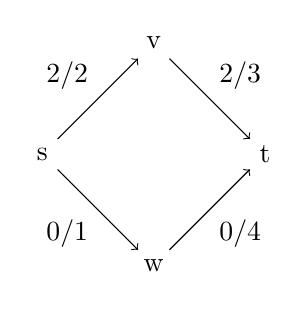
\begin{tikzpicture}[node distance = 2cm, auto]
 \node (v) {v};
 \node (s) [below left of=v] {s};
 \node (w) [below right of=s] {w};
 \node (t) [below right of=v] {t};

 \path [->] (v) edge node[above right]{2/3} (t);
 \path [->] (s) edge node[above left] {2/2}(v);
 \path [->] (s) edge node[below left] {0/1} (w);
 \path [->] (w) edge node[below right] {0/4} (t);
\end{tikzpicture}
\end{center}
Der Restgraph mit Restkapazitäten ist:
\begin{center}
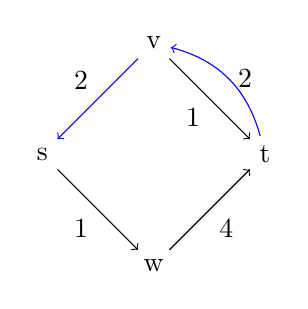
\begin{tikzpicture}[node distance = 2cm, auto]

	\node (v) {v};
 \node (s) [below left of=v] {s};
 \node (w) [below right of=s] {w};
 \node (t) [below right of=v] {t};
\begin{scope}[every edge/.style={draw=blue}]
 \path [->] (t) edge[bend right=30] node[right] {2} (v);
 \path [<-] (s) edge node[above left] {2}(v);
 \end{scope}
 \begin{scope}[ever edge/.style={draw=red}]
 \path [->] (s) edge node[below left] {1} (w);
 \path [->] (w) edge node[below right] {4} (t);
 \path [->] (v) edge node[below left]{1} (t);
\end{scope}
\end{tikzpicture}
\end{center}
Blau: Rückwärtskante, Rot: Vorwärtskante
\end{example}
Der Beweis von Satz \ref{thm:min-cut} gibt uns außerdem einen Algorithmus, wie wir, für einen nicht-optimalen Fluss, ein Fluss mit höheren Wer finden können.
\underline{Idee:} Benutze dies um einen optimalen Fluss zu finden. \\
\begin{algorithm}[H]
	\label{alg:ford-fulkerson}
	\caption{Ford-Fulkerson}
	\KwData{Netzwerk $N=(V,E,c,s,t)$ }
	\KwResult{Fluss $f$ mit $flow(f)=MaxFlow(N)$ }
	\begin{itemize}
		\item $f(e)=0, e \in E$ 
		\item Suche einen augmentierenden Weg von $s$ nach $t$ 
		\item \If{ keiner existiert}{stop}
		\item Berechne $\varepsilon$ \eqref{eqn:epsilon}
		\item Augmentiere $f$ um $\varepsilon$, gehe zu 2
	\end{itemize}
\end{algorithm}
\begin{remark}
Im Falle von irrationalen Kapazitäten muss der Algorithmus nicht notwendigerweise terminieren (Beweis durch Gegenbeispiel)
\end{remark}
\begin{theorem}[Integral-Flow-Theorem]
Sei $N=(V,E,c,s,t)$ ein Netzwerk mit ganzzahligen Kapazitäten. Dann terminiert der Algorithmus \ref{alg:ford-fulkerson} nach maximal $\sum_{e \in E}c(e)$ Augmentierungsschritten mit einem ganzzahligen, optimalen Fluss.
\end{theorem}
\begin{proof} Betrachte:
\paragraph{Ganzzahlig:} Wir starten mit $f(e)=0, e \in E$. Die Restkapazitäten im Algorithmus und somit auch $\varepsilon $ sind zu jedem Zeitpunkt ganzzahlig.
\paragraph{Optimal:} Der Algorithmus terminiert, falls kein augmentierender Weg mehr gefunden werden kann. Der Beweis des Max-Flow-Min-Cut-Theorem zeigt, dass dies den maximalen Fluss impliziert.
\paragraph{Anzahl Schritte} Im schlimmsten Fall wird pro Iteration der Fluss von genau einer Kante um 1 erhöht $\implies$ Behauptung 
\end{proof}
%Beispiel

Es gibt eine Möglichkeit, die Laufzeit des Algorithmus zu verbessern, indem man immer den kürzesten augmentierenden Weg wählt. Dies bringt uns zum nächsten Algorithmus: \\
\begin{algorithm}[H]
	\label{alg:edmonds-karp}
	\caption{Edmonds-Karp}
	\KwData{Netzwerk $N=(V,E,c,s,t)$}
	\KwResult{Fluss $f$ mit $flow(f)=MaxFlow(N)$}
	\begin{itemize}
		\item $f(e)=0, e \in E$ 
		\item Suche einen kürzesten augmentierenden Weg von $s$ nach $t$
		\item \If{keiner existiert}{stop}
		\item Berechne $\varepsilon$ \eqref{eqn:epsilon}
		\item Augmentiere $f$ um $\varepsilon $ und gehe zu 2
	\end{itemize}
\end{algorithm}
\begin{example}
Betrachte
%Grafik auf Vorlesung 19 Seite 2 muss hinzugefügt werden
\end{example}
\begin{lemma}
	Sei $(f_0,\pi_0),(f_1,\pi_1)\ldots$ die Folge von Flüssen $f_i$ mit zugehörigen augmentierenden Weg $\pi $, die vom Edmonds-Karps-Algorithmus \ref{alg:edmonds-karp} erzeugt wird. Dann gilt:
	\[
	|\pi_i \le |\pi_{i+1}| \text{ für alle } i
	\]
und falls $e=(v,w)$ in $\pi_i $ und $e^{-1}=(w,v)$ in $\pi_j,  i<j$ dann gilt:
\[
|\pi_i| +2 \le |\pi_j|
\]
\end{lemma}
\begin{proof}
	%Sind das Gs oder fs?
Sei $l_i(x,y)$ die Länge des kürzesten x-y-Wegs im Restgraphen von $f_i \implies |\pi_i|=e_i(s,t)$ \\
\underline{Behauptung 1} $l_{i+1}(s,v) \ge l_i(s,v)$ für alle $v \in V$ \\
Falls $l_{i+1}(s,v)=\infty$ ist Behauptung 1 trivial. \\
Sonst: $v$ ist von $s$ im Restgraphen von $f_{i+1}$ erreichbar, d.h
\[
\infty>l_{i+1}(s,v)=r
\]
Sei also $\pi=s,v_1,\ldots,v_r$ ein kürzester Weg von s nach $v=v_r$ im Restgraphen von $f_{i+1}$. \\
\underline{Behauptung 2 } $l_i(s,v_{j+1}) \le l_i(s,v_j)+1, 1\le j<r$ \\
\begin{proof}
Behauptung 2
\begin{itemize}
	\item \emph{Fall 1} $(v_j,v_{j+1})$ hat eine Kante im Restgraphen $f_i \to$ trivial
	\item \emph{Fall 2} $(v_j,v_{j+1})=e$ ist keine Kante im Restgraphen von $f_i$.
		\begin{align*}
		&\implies e^{-1}=(v_{j+1},v_j) \text{ ist Kante im Restgraphen von } f_i \\
		&\implies \text{ Der Flusswert von} e^{-1} \text{ muss sich von } f_i \text{ zu } f_{i+1} \text{ verändert haben.} \\
		&\implies (v_{j+1}),v_j) \text{liegt auf }\pi_i \\
		&\implies l_i(s,v_{j+1}) =l_i(s,v_j) -1 \le l_i(s,v_j)+1
		\end{align*}
\end{itemize}
\end{proof}
\begin{proof}
Behauptung 1. Rechne:
\begin{align*}
	l_i(s,v) &= l_i(s,v_r) \\
		 &\le  l_i(s,v_{r-1}) +1 \\
		 &\le \ldots \\
		 &\le l_i(s,s) +r \\
		 &= l_{i+1}(s,v)
\end{align*}
Behauptung 1 impliziert 1. mit $v=t$. 
\end{proof}
\underline{Behauptung 3} $l_{i+1} (v,t) \ge l_i(v,t)$ für alle $i$ \\
Beweis Analog zu Behauptung 1. \\
Nun können wir alles zusammenführen und rechnen:
\begin{align*}
	|\pi_j| &= l_j(s,t) \\
		&= l_j(s,w) +1 +l_j(v,t) \\
		&\ge l_i(s,w) +1 + l_i(v,t) \\
		&= l_i(s,v) + l_i(v,t) +2 \\
		&= |\pi_i|+2
\end{align*}
\end{proof}
\begin{theorem}
	Der Algorithmus von Edmonds-Karp \ref{alg:edmonds-karp} terminiert nach höchsten $\frac{m\cdot n}{2}$ Augmentierungsschritten, $m=|E|, n=|V|$. 
\end{theorem}
\begin{proof}
Sei $(f_0,\pi_0),(f_1,\pi_1),\ldots$ die vom Algorithmus erzeugte Folge von Flussfunktionen $f_i$  und zugehörigen augementierenden Wegen $\pi_i$ im Restgraphen von $f_i$ .\\
\emph{Beobachte 1:} In jedem Augmentierungsschritt wird mindestens eine Kante $e \in (v,w)$  in $\pi_i$ voll ausgeschöpft:
\begin{itemize}
	\item $e$ Vorwärtskante  im Restgraph zu $f_i$
		\[
		f_i(e) < c(e) \to f_{i+1}(e)=c(e)
		\]
	\item e Rückwärtskante im Restgraph zu $f_i$ 
		\[
		f_i(e)>0 \to f_{i+1}(e) = 0
		\]
\end{itemize}
$\implies e$ ist im $i+1$ Schritt nicht im Restgraph. \\
\emph{Beobachte 2:} In Augmentierungsschritt $f_k \to f_{k+1}$ kann $e$  nur in $\pi_k$ vorkommen und voll ausgeschöpft werden, falls $e^{-1}=(w,v)$ im Weg $\pi_j, i<j<k$ vorgekommen ist. 
\[
	\implies |\pi_i|\le |\pi_j| -2 \le |\pi_k| -4
\]
\underline{Also:} Falls $e$ in $\pi_{i_0},\ldots,\pi_{i_e}$ voll ausgeschöpft wird, gibt es $j_0,\ldots,j_{e-1}$ so, dass
\begin{itemize}
	\item $i_0<j_0<i_1<j_1<\ldots<j_{e-1} < i_{e}$
	\item $e^{-1}$ kommt in $\pi_{j_0},\ldots,\pi_{j_{e-1}}$ vor
	\item $1 \le |\pi_{i_0}| \le \ldots\le |\pi_{i_k}|-4l$ 
\end{itemize}
\emph{Beobachte:} $\pi_{i_k}$ ist eine kürzester Weg im Restgraphen von $f_{i_k}$
\begin{align*}
&\implies \pi_{i_k} \text{ ist einfach}\\
&\implies |\pi_{i_k}| <n \\
&\implies l< \frac{n}{4} \text{ für jede Kante}\\
&\implies \text{ maximal } 2m \frac{n}{4}= \frac{m\cdot n}{2} \text{ Augmentierungsschritte}
\end{align*}
\end{proof}
\begin{remark}
Dies beweist die Existenz einer Lösung des Netzwerkflussproblems  für Kapazitäten in $R_{\ge  0}$. 
\end{remark}
\begin{corollary}
	Für $m=|E|, n=|V|,$ ist der Aufwand des Edmonds-Karp Algorithmus $\mathcal{O}(m^2n)$. 
\end{corollary}
\begin{proof}
Ein kürzeste-Wege-Problem pro Schritt lösbar in $\mathcal{O}(m)$ mit Breitensuche.  
\end{proof}


\addchap{Numerische Lösung linearer Gleichungssysteme}
\section*{Motivation}
Für $\K \in \{\R, \C \}$ bezeichnen wir $\K^{n}$ den Vektorraum der  $\K$-wertigen Vektoren 
\[
\vec{x}=\begin{pmatrix} x_1 \\ \vdots \\ x_n \end{pmatrix}, x_{i}\in \R, i=1,\ldots,n
\]
und mit $\K^{m\times n}$ den Vektorraum der $\K$-wertigen Matrizen 
\[
A= \begin{bmatrix}
	a_{1,1} & \ldots & a_{1,n} \\

	\vdots & & \vdots \\
	a_{m,1} & \ldots & a_{m,n}
\end{bmatrix}, a_{i,j} \in \K, i=1,\ldots,m , j=1,\ldots,n
\]
In vielen Anwendungen in Physik, Ökonomie, Life Sciences, Informatik, etc.
müssen lineare Gleichungssysteme gelöst werden, also System der Form:
\[
Ax=b, A \in \R^{n\times n}, x,b \in \R^{n}
\]
Hierbei ist n oft sehr groß.

\section{Vektoren- und Matrixnormen}

Im folgendem werden wir uns damit beschäftigen, ob lineare Gleichungssysteme gut oder schlecht konditioniert sind, d.h kann man stabile Algorithmen zur Lösung solcher Systeme zur Lösung angeben.

\begin{definition}
Sei $X$ ein $\K$-Vektorraum. Eine Abbildung $\|•\| \colon X \to (0,\infty) $ heißt \emph{Norm} auf $X$, falls:
\begin{enumerate}
	\item $\|x\|>0$ für alle $x \in X \setminus \{0\}$
	\item $\| \alpha \cdot x \|= |\alpha| \cdot \|x\|$ für alle $\alpha \in \R, x \in X$
	\item $\|x+y\|\le \|x\|+\|y\|$, für alle $x,y \in X$ 
\end{enumerate}
\end{definition}
\begin{remark}
Jede Norm induziert auch einen Distanzbegriff, den durch die Norm induzierte Metrik 
\[
dist(x,y)=\|x-y\|
\]
Wegen $x=x-0$ kann $\|x\|$ deshalb als Distanz zum Nullpunkt aufgefasst werden, welche von der gewählten Norm abhängt.  
\end{remark}
\begin{example}Normen:
\begin{itemize}
	\item Für $X= \K^{n}$
		\begin{itemize}
			\item Betragssummennorm: $\|x\|_1 = \sum_{i=1}^{n}|x_{i}|$
			\item Euklidische Norm: $\|x\|_2 = \sqrt[2]{\sum_{i=1}^{n}|x_{i}|^2} $ 
			\item Maximumsnorm: $\|x\|_{\infty} = \max_{1\le i\le n} |x_{i}|$ 
			\item Schatten p-Norm- $\|x\|_p = \sqrt[p]{\sum_{i=1}^{n}|x_{i}|^{p}} $ 
		\end{itemize}
	\item Für $X = \K^{m\times n}$ 
		\begin{itemize}
			\item Spaltensummennorm: $\|A\|_1 = \max_{1\le j\le n} \sum_{i=1}^{m}|a_{i,j}|$ 
		\item Zeilensummennorm: $\|A\|_{\infty} = \max_{1\le i\le m} \sum_{j=1}^{n}|a_{i,j}|$
		\item Frobeniusnorm $\|A\|_F = \sqrt[2]{\sum_{i=1}^{m}\sum_{j=1}^{n}|a_{i,j}|^2}$ 
		\end{itemize}
\end{itemize}
Für $A = \begin{bmatrix}
	2  & -3 \\
	1 & 1 
\end{bmatrix}$
gilt: 
\[
\|A\|_1=4 , \|A\|_{\infty} = 5, \|A\|_F = \sqrt[2]{15} 
\]
\end{example}

\begin{theorem}
	Alle Normen auf $\K^{n}$ sind äquivalent, d.h für zwei Normen $\|•\|_a, \|•\|_b$ auf $\K^{n}$ gilt:
	\[
	\underline{c} \|x\|_a \le \|x\|_b\le \overline{c}\|x\|_a
	\]
für $\underline{c},\overline{c}>0$, unabhängig von $x$. 
\end{theorem}
\begin{proof}
Es genügt die Behauptung für $\|•\|_a = \|•\|_{\infty}$  und $\|•\|_b$  beliebig zu zeigen. Wegen:
\[
x-y = \sum_{i=1}^{n}(x_{i}-y_{i}) e_i
\]
gilt:
\begin{align*}
	\lvert \|x\|-\|y\|\rvert &\le  \|x-y\| \\
				 &= \|\sum_{i=1}^{n}(x_{i}-y_{i}) e_i\| \\
				 &\le \sum_{i=1}^{n}\|(x_{i}-y_{i})e_i\| \\
				 &= \sum_{i=1}^{n}|x_{i}-y_{i}| \|e_i\| \\
				 &\le \|x-y\|_{\infty} \sum_{i=1}^{n}\|e_i\|
\end{align*}
Also ist $\|•\| \colon \K^{n} \to \R $ eine Lipschitz-stetige Funktion mit Konstante L. \\
$\implies \|•\|$ nimmt auf jeder kompakten Menge sowohl Minimum $\underline{c}$ als auch Maximum $\overline{c}$ an. Insbesondere auch auf:
\[
S^{n-1} = \{x \in \K^{n} : \|x\|_{\infty} =1\} 
\]
\begin{align*}
&\implies 0 < \underline{c} \le \overline{c} \\
&\implies \underline{c} \le \|\frac{x}{\|x\|_{\infty}}\|\le \overline{c} \\
&\implies \underline{c} \|x\|_{\infty} \le \|x\| \le \overline{c}\|x\|_{\infty}
\end{align*}
\end{proof}
\begin{corollary}
	Analog für Matrizen.
\end{corollary}
\begin{example}
Für $x \in \K^{n}$
\[
\|x\|_{\infty}^2 = \max_{1\le i\le n} |x_i|^2 \le \sum_{i=1}^{n}|x_{i}|^2 \le n \max |x_{i}|^2 = n \cdot  \|x\|_{\infty}^2
\]
$\implies \|x\|_{\infty} \le \|x\|_2 \le \sqrt[2]{n} \|x\|_{\infty}$ \\
Die deutet darauf hin, dass im Unendlichdimensionalen nicht alle Normen äquivalent sind.
\end{example}
Da Matrizen miteinander multipliziert werden können, können Normen auf Matrizen spezielle Eigenschaften haben, die diese Eigenschaft wiederspiegeln.

\begin{definition}
Eine Matrixnorm $\|•\|_M$ heißt \emph{submultiplikativ}, falls 
\[
\|A\cdot B\|_M \le \|A\|_M \cdot \|B\|_M
\]
für alle $A,B \in \K^{n\times n}$.\\
Eine Matrixnorm $\|•\|_M$ auf $\K^{n\times n}$ heißt \emph{verträglich} mit einer Vektornorm $\|•\|_V$  auf $\K^{n}$ , falls:
\[
\|Ax\|_V \le \|A\|_M \cdot \|x\|_V
\]
für alle $A \in \K^{n\times n}, x \in \K^{n}$ .
\end{definition}
\begin{example}
\begin{itemize}
	\item $\|A\|= \max |a_{i,j}$ ist nicht submultiplikativ auf $\K^{n\times n}$.
		\[
		A = \begin{bmatrix}
		 1 & 1 \\ 1 & 1
		\end{bmatrix} \implies \|A\|=1
		\]
		jedoch 
		\[
		A^2= \begin{bmatrix}
			2 & 2 \\ 2 & 2
		\end{bmatrix} \implies \|A^2\|=2 \neq 1 = \|A\|^2
		\]
	\item Die Frobenius Norm ist submultiplikativ und mit der Euklischen Norm verträglich (Übung)
\end{itemize}
\end{example}
\begin{definition}
Sei $\|•\|_V $ eine Vektornorm auf $\K^{n}$ , dann ist 
\[
|\|A\|| = \sup_{x\neq 0} \frac{\|Ax\|_V}{\|x\|_V}= \max \|Ax\|_V
\]
eine Norm auf $\K^{n\times n}$, die von  $\|•\|_V$ induzierte Matrixnorm. 
\end{definition}
\begin{example}
Die Spaltensummennorm ist von $\|•\|_1$ und die Zeilensummennorm ist von $\|•\|_{\infty}$ induziert.
\end{example}
\begin{lemma}
	Die von $\|•\|_V$ induzierte Matrixnorm ist submultiplikativ und ist mit $\|•\|_V$ verträglich. Ist $\|•\|_M$ eine mit $\|•\|_V$ verträgliche Matrixnorm so gilt:
	\[
	|\|A\|| \le \|A\|_M
	\]
	für alle $A \in \K^{n\times n}$ .
\end{lemma}
\begin{proof}
Unterteile:
\paragraph{Submultiplikativität} $A=0$ oder $B=0 \implies$ klar. \\
Seien $A,B \neq 0$:
\begin{align*}
	|\|AB\|| 
	&= \sup_{x\neq 0} \frac{\|ABx\|_V}{\|x\|_V} \\
	&= \sup_{Bx\neq 0} \frac{\|ABx\|_V}{\|x\|_V} \\
	&= \sup_{Bx \neq 0} \left( \frac{\|ABx\|_V}{\|x\|_V} \frac{\|Bx\|_V}{\|x\|_V} \right) \\
	&\le \left( \sup_{Bx \neq 0} \frac{\|ABx\|_V}{\|x\|_V} \right) \left( \sup_{Bx\neq 0} \frac{\|Bx\|_V}{\|x\|_V} \right) \\
	&= |\|A\|| \cdot |\|B\||
\end{align*}
\paragraph{Verträglichkeit} $A= 0$ oder $x=0$  klar. \\
Seien $A \neq 0, x\neq 0$. 
\begin{align*}
&\implies \frac{\|Ax\|_V}{\|x\|_V} \le \sup \frac{\|Ax\|_V}{\|x\|_V} = |\|A\|| \\
&= \text{ Behauptung.}
\end{align*}
Rechne nun: 
\[
|\|A\|| = \sup \frac{\|Ax\|_V}{\|x\|_V}\le  \|A\|_M
\]
da $\|Ax\|_V \le \|A\|_M \|x\|_v$ 
\end{proof}
\begin{remark}
Mit den offensichtlichen Modifikationen gelten die Definitionen über Submultiplikativität und Verträglichkeit auch für rechteckige Matrizen.
\end{remark}

\section{Kondition linearer Gleichungssysteme}
\begin{recall}
Die Kondition beschreibt, wie sehr Fehler in den Eingangsdaten eines Problems
verstärkt oder gedämpft werden und sich auf einen Fehler der Ausgangsdaten übertragen.
\end{recall}
Zum Lösen von $Ax=b$, $A$ invertierbar, bezeichnen wir $\Delta b$ als einen Eingangsfehler in $b$. 
\begin{align*}
&\implies x+ \Delta x = A^{-1}(b+\Delta b) = A^{-1}b +A^{-1} \Delta b \\
&\implies \Delta x= A^{-1} \Delta b
\end{align*}
Für ein verträgliches Matrix-Vektorraum-Paar gilt dann: 
\[
\|\Delta x\|= \|A^{-1} \Delta b\| \le \|A^{-1}\|\|\Delta b\| 
\]
und 
\[
	\frac{\|\Delta x\|}{\|x\|} \le \|A^{-1}\| \frac{\|\Delta b\|}{\|x\|}\le  \|A^{-1}\| \|A\| \frac{\|\Delta b\|}{\|b\|}
\]
\begin{definition}
Der Faktor 
\[
cond_M (A) = \|A^{-1}\|_M \|A\|_M 
\]
wird als \emph{Kondition} der Matrix $A$ bezüglich der Matrixnorm $\|•\|_M$ bezeichnet. 
\end{definition}
\begin{example}
	\label{eg:lgs-kondition}
Betrachte 
\[
A= \begin{bmatrix}
	10^{-3} & 1 \\
	1 & 1
\end{bmatrix}
\]
\begin{align*}
	&\implies A^{-1} \approx \begin{bmatrix}
		-1.001 & 1.001 \\
		1.001 & -0.001
	\end{bmatrix} \\
	&\implies \|A\|_{\infty} =2 & \|A^{-1}\|_{\infty} \approx 2 \\
	&\implies cond_{\infty}(A) \approx 4
\end{align*}
A ist also bezüglich $\|•\|_{\infty}$ gut konditioniert.
\end{example}

\section{LR-Zerlegung}
Man betrachte das Lösen von linearen Gleichungssystemen
\begin{align*}
\begin{bmatrix}
	a_{1,1} & \ldots a_{1,n} \\
	\vdots & & \vdots \\
	a_{n,1} & \ldots & a_{n,n}
\end{bmatrix}
\cdot 
\begin{bmatrix}
	x_1  \\ \vdots \\ x_{n}
\end{bmatrix}
=
\begin{bmatrix}
	b_1 \\ \vdots \\_{n}
\end{bmatrix}
\end{align*}
mittels Gauss-Elimination. Im i-ten Schritt:
\begin{align*}
\begin{gmatrix}[b][ccccc|c]
	* & \ldots & \ldots &\ldots& *  &*\\
	0 & * & \ldots &\ldots& * &*\\
	\vdots  & 0 & a_{i,i}^{(i)} & \ldots & a_{i,n}^{(i)}  & b_i^{(i)} \\
	\vdots & \vdots & \vdots &  & \vdots  &  \vdots\\
	0 & 0 & a_{n,i}^{(i)} & \ldots & a_{n,n}^{(i)} &  b_n^{(i)}
\rowops
\mult{2}{\cdot(-\tau_{i+1}^{(i)})}
\add{2}{3}
\mult{2}{\cdot(-\tau_{n}^{(i)})}
\add{2}{4}
\end{gmatrix}
&
\tau_j^{(i)}= \frac{a_{j,i}^{(i)}}{a_{i,i}^{(i)}}
\end{align*}\\[2ex]
Die Elimination im i-ten Schritt lässt sich als Matrix-Matrix-Produkt darstellen:
\[
L_i [A_i | b_i] = [A_{i+1} | b_{i+1}]
\]
wobei 
\begin{align*}
	L_i = \begin{bmatrix}
		  1 & & & & \\
		  & 1 & & & \\
		  & & 1 & & \\
		  & & -\tau_{i+1}^{(i)}& 1 & \\
		  & & -\tau_n^{(i)}& & 1
	\end{bmatrix}
\end{align*}
In der Matrix-Schreibweise ist der Gauss-Algorithmus also als
\[
L_{n-1}\cdot L_{n-2} \cdot \ldots \cdot L_1[A|b] = [A_n|b_n] = [R|c] = \begin{bmatrix}
	* & \ldots & * \\
	  & \ddots  & \vdots \\
	0  &   & *
\end{bmatrix}
\]
darstellbar, wobei R eine \emph{obere Dreiecksmatrix} ist. \\
Insbesondere folgt aus 
\[
L_{n-1} \cdot  \ldots \cdot L_1 A = R \text{,}
\]
dass
\[
A= L_1^{-1} \ldots L_{n-1}^{-1} R = LR
\]
ist.

\begin{lemma}
	Es gilt:
	\begin{enumerate}
		\item $L_i = I-l_i e_i^{t} = I- \begin{bmatrix}
		0 \\ \vdots \\ 0 \\ \tau_{i+1}^{(i)} \\ \vdots \\ \tau_n^{(i)}
		\end{bmatrix}$ 
		\item $L_i^{-1} = I+ l_i e_i^{t} = \begin{bmatrix}
			1 & & & & \\
                  & 1 & & & \\
                  & & 1 & & \\
                  & & -\tau_{i+1}^{(i)}& 1 & \\
                  & & -\tau_n^{(i)}& & 1
		\end{bmatrix}$
	\item $L= I+ l_1e_1^{t}+ l_2^{t}e_2+\ldots+ l_{n-1} e_{n-1}^{t}= \begin{bmatrix}
			1 & \\
			\tau_2^{(1)} & 1 \\
			\tau_3^{(1)} & \tau_3^{(2)} & 1 \\
			\vdots & \vdots & \ddots & \ddots \\
			\tau_n^{(1)} & \tau_n^{(2)} &  \ldots &\tau_n^{n-1} & 1
	\end{bmatrix}$ 
	\end{enumerate}

\end{lemma}
\begin{proof} Nacheinander:
\begin{enumerate}
	\item Durch hinschreiben.
	\item Rechne: 
		\[
			(I-l_i e_i^{t}) (I+l_ie_i^{t}) = [\ldots 1 \ldots] \cdot \begin{bmatrix}
				0 \\ \vdots \\ 0 \\ * \\ \vdots \\ *
			\end{bmatrix} = 0 
		\]
	\item Zeige per Induktion über i, dass: $L_1^{-1} \ldots L_i^{-1} = I + l_1e_1^{t} + \ldots + l_ie_i^{t}$
		\begin{itemize}[label=$\lozenge$, itemsep=2ex]
			\item IV \underline{$i=1$} aus b.
			\item IS \underline{$i \to i+1$} 
			\begin{align*}
			L_1^{-1} \ldots L_i^{-1} L_{i+1}^{-1} &= (I+ l_1e_1^{t}+\ldots+ l_ie_i^{t}) (I+l_{i+1} e_{i+1}^{t}) \\
	&= I + l_1e_1^{t}+l_2e_2 + \ldots + l_ie_i^{t}+ l_{i+1}e_{i+1}^{t}
			\end{align*}
		\end{itemize}
\end{enumerate}
\end{proof}
Wir können L also direkt aus den im Gauss-Algorithmus vorkommenden Größen zusammensetzen. Der Algorithmus bricht ab, wenn eins der Pivotelemente null wird.

\begin{theorem}
	Falls kein Pivotelement null wird, bestimmt der Gauss-Algorithmus neben der Lösung $x$ von $Ax=b$ eine LR-Zerlegung $A=LR$ in eine obere Dreiecksmatrix $R$ und eine normierte, untere Dreiecksmatrix $L$.
\end{theorem}
\begin{example}
	\label{eg:gauss}
Betrachte den Gauss-Algorithmus angewandt auf:
\begin{align*}
	A &=
\begin{gmatrix}[b]
1 & 4 & 7\\
2 & 5 & 8\\
3 & 6 & 10
\rowops
\mult{0}{-2}
\add{0}{1}
\mult{0}{-3}
\add{0}{2}
\end{gmatrix} \\
	  &\to \begin{gmatrix}[b]
1 & 4 & 7\\
0 & -3 & -6\\
0 & -6 & -11
\rowops
\mult{1}{-2}
\add{1}{2}
\end{gmatrix} \\
	  &\to \begin{gmatrix}[b]
1 & 4 & 7\\
0 & -3 & -6\\
0 & 0 & 1
\end{gmatrix}=R
	  &L = \begin{bmatrix}
		  1 & 0 & 0 \\
		  2 & 1 & 0 \\
		  3 & 2 & 1
	  \end{bmatrix}
\end{align*} 
\end{example}
\begin{remark}
In der Praxis werden die ursprünglichen Einträge der Matrix $A$ durch die modifizierten Einträge $a_{i,j}^{(k)}$ überschrieben. Die Matrix $L$ lässt sich sukzessive in die nicht mehr benötigten untere Hälfte von A schreiben. Man spricht von "in place"- Algorithmen, die keinen zusätzlichen Speicher benötigen.
\end{remark}
Mit Hilfe der LR-Zerlegung wollen wir im folgenden das Lösen von linearen Gleichungssystemen ermöglichen.
\begin{description}
	\item[1] Berechne $A=LR$
	\item [2] Löse $Ax=LRx=b$ durch
		\begin{itemize}
			\item Löse $Ly =b $ mittels Vorwärtssubstitution
			\item Löse $Rx=y$ mittels Rückwärtssubsititution
		\end{itemize}
\end{description}
\begin{algorithm}[H]
	\label{alg:subsitution}
	\caption{Vorwärts- und Rückwärtssubsitution}
	\KwData{LR-Zerlegung $A=LR$ invertierbar, $A \in \R^{n\times n}, b \in \R^{n}$}
	\KwResult{Lösung $x$ von $Ax=b$ }
\For {$i \gets 1$ \KwTo $n$}{$y_i= b_i - \sum_{j=1}^{i-1}L_{i,j}y_j$}
\For {$i \gets n$ \KwTo $1$}{$x_i = \frac{1}{R_{i,i}}\left( y_i - \sum_{j=i+1}^{n}R_{i,j}x_j \right) $} 
\end{algorithm}
\begin{example}
Löse $Ax=b$ mit $A$ aus Beispiel \ref{eg:gauss}: 
\begin{align*}
	A &= \begin{bmatrix}
		1 & 4 & 7 \\
		2 & 5 & 8 \\
		3 & 5 & 10 
	\end{bmatrix} = \begin{bmatrix}
	1 \\
	2 & 1 \\
	3 & 2 & 1
	\end{bmatrix}
	\cdot
	\begin{bmatrix}
		1 & 4 & 7 \\
		  & -3 & -6 \\
		  & & 1
	\end{bmatrix}
	  & 
	b= \begin{bmatrix}
	1 \\ 1 \\ 1
	\end{bmatrix}
\end{align*}
Vorwärtssubstitution: 
\begin{align*}
Ly= \begin{bmatrix}
	1 \\
	2 & 1 \\
	3 & 2 & 1
\end{bmatrix}
\cdot 
\begin{bmatrix}
y_1 \\ y_{2} \\ y_3 
\end{bmatrix}
= 
\begin{bmatrix}
1 \\ 1 \\ 1
\end{bmatrix} =b 
&\implies \begin{cases}
	y_1=1 \\
	y_2= 1-2 =-1 \\
	y_3= 1-3-2\cdot (-1) =0
\end{cases}
\end{align*}
Rückwärtssubstitution:
\begin{align*}
	Rx= \begin{bmatrix}
		1 & 4 & 7 \\
		  & -3 & -6 \\
		  & & 1
	\end{bmatrix}
	\cdot 
	\begin{bmatrix}
	x_1 \\ x_2 \\ x_3
	\end{bmatrix}
	= \begin{bmatrix}
	1 \\ -1 \\ 0
	\end{bmatrix} = y
	&\implies \begin{cases}
		x_3 = 0 \\
		x_2= \frac{1}{-3}(-1-(-6) 0) =\frac{1}{3} \\
		x_1= 1(1-\frac{4}{3}-7\cdot 0 = -\frac{1}{3}
	\end{cases}
\end{align*}
\end{example}
\begin{remark}
Die LR-Zerlegung und Vorwärts- und Rückwärtssubstitution sind zum klassischen Gauss-Algorithmus äquivalent, es werden sogar die genau gleichen Operationen durchgeführt. Die LR-Zerlegung kann jedoch für andere rechte Seiten wiederverwendet werden.
\end{remark}
\paragraph{Aufwand:} Anzahl der Multiplikationen im i-ten Schirtt:
\[
n-i + (n-i) (n-i) = (n-i)^2 + n-i
\]
Also 
\[
\sum_{i=1}^{n-1}\left( (n-i)^2 + n-i \right)= \sum_{i=1}^{n-1}\left( i^2+i \right)= \frac{1}{3}n^3 + \mathcal{O}(n^2)
\]
Multiplikationen zur Berechnung der $LR$-Zerlegung.
Der Aufwand der Substitutionen beträgt: $\mathcal{O}(n^2)$. \\
Daraus resultiert ein Gesamtaufwand zum Lösen eines linearen Gleichungssystem von : $\frac{1}{3}n^3+\mathcal{O}(n^2)$. Der Aufwand im Speicher ist $\mathcal{O}(n^2)$.
%missing Charamsche Regel, cause not important.

\section{LR-Zerlegung mit Spaltenpivotisierung}
\begin{example}
	Fortsetzung von Beispiel \ref{eg:lgs-kondition}
	\begin{align*}
	A= \begin{bmatrix}
		10^{-3} & 1 \\
		1 & 1
	\end{bmatrix}
	&, b= \begin{bmatrix}
	1 / 2
	\end{bmatrix}
	&\implies x = \begin{bmatrix}
	1.001001 \\ 0.998999
	\end{bmatrix}
	\end{align*}
	Löse in dreistelliger Arithmetik, mit kleiner Störung in der rechten Seite:
	\begin{align*}
	\begin{gmatrix}[b]
		0.001 & 1 & 1.01\\
		1 & 1 & 2.01
\rowops
\mult{0}{-1000}
\add{0}{1}
\end{gmatrix}
&\to \begin{bmatrix}[cc|c]
	0.001 & 1 & 1.01 \\
	0 & -999 & -1010
\end{bmatrix}
\\ 
&\implies \begin{cases}
	x_2= -1010 \boxslash (-999) = 1.01 \\
	x_1= (1.01 \boxminus (1 \boxcircle 1.01)) \boxslash 0.001 = 0
\end{cases}
	\end{align*}
Der Algorithmus muss also instabil sein.
\end{example}
\paragraph{Grund:} Das Inverse des Pivot-Elemts (1000) ist sehr groß und verstärkt den Fehler

\begin{definition}
	Sei $1\le i < j \le n$
	\begin{align*}
	T^{\{i,j\}} = \begin{bmatrix}
		1 \\
		& \ddots\\
		& & 1 \\
		& & & 0 & & & & 1\\
		& & & & 1 \\
		& & & & & \ddots\\
		& & & & & & 1\\
		& & & 1 & & & & 0 & \\
		& & & & & & & & 1 \\
		& & & & & & & & & \ddots \\
		& & & & & & & & & &  1
	\end{bmatrix}
	\end{align*}
	heißt Transpositionsmatrix.\\
	Eine Permutationsmatrix ist das Produkt mehrerer Transpositionsmatrizen.
	\end{definition}

\begin{lemma}
	Sei $T^{\{i,j\} }$ eine Transpositionsmatrix. Es gilt:
	\begin{enumerate}
		\item Multiplikation von links mit $T^{\{i,j\} }$ vertauscht i-te und j-te Zeile.
		\item Multiplikation von rechts mit $T^{\{i,j\} }$ vertauscht i-te und j-te Spalte. 
		\item $T^{\{i,j\} }$  ist symmetrisch. 
		\item $\left( T^{\{i,j\} } \right)^2=I$ 
	\end{enumerate}
	Ist $P$ eine Permutationsmatrix, so gilt: $P^{T}P=I$ 
\end{lemma}
\begin{proof}
a-d sind elementar. Letzter Punkt: Übung.
\end{proof}
\paragraph{Umseztung:} Anstatt im i-ten Schritt des Gauss-Algorithmus 
\[
A_i \to L_iA_i =A_{i+1}
\]
zu berechnen, berechnen wir:
\begin{equation}
\label{eqn:lr-gauss}
A_i \to  L_iP_iA_i = A_{i+1}
\end{equation}
\begin{lemma}
	Sei $1 \le i < j \le n$ und $P_i = T^{\{i,k\} }$ mit $i<k\le n$. Dann gilt: $P_iL_j=\tilde{L_j}P_i$, wobei $\tilde{L_j}$ und $L_j$ bis auf ein Vertauschen der $\tau_k^{(j)}$ und $\tau_i^{(j)}$ gleich sind.  
\end{lemma}
\begin{proof}
Durch nachrechnen. Also:
\[
\tilde{L_j} = P_iL_jPi
\]
\end{proof}
\begin{theorem}
	Sei A nicht singulär. Dann bestimmt der Gauss-Algorithmus mit Spaltenpivotisierung eine Zerlegung der Matrix $PA=\tilde{L}R$ , wobei $R$ die obere Dreiecksmatrix $A_n$ ,$P=P_{n-1} \ldots P_1$ eine Permutationsmatrix und $\tilde{L} = \tilde{L_1^{-1}}\ldots\tilde{L_{n-1}^{-1}}$ eine untere Dreiecksmatrix ist mit:
	\begin{align*}
		&\tilde{L_{n-1}} = L_{n-1} \\
		&\tilde{L_{n-2}} = P_{n-1} L_{n-2} P_{n-1} \\
		&\ldots  \ldots\\
		&\tilde{L_1}= P_{n-1}P_{n-2}\ldots P_2P_1 L_1 P_2 \ldots P_{n-2} P_{n-1}
	\end{align*}
\end{theorem}
\begin{proof}
Falls der Algorithmus nicht zusammenbricht:
\begin{align*}
	R = A_n &= L_{n-1} P_{n-1} A_{n-1} \\
		&= \tilde{L_{n-1}} P_{n-1} L_{n-2} P_{n-2} A_{n-2} \\
		&= \tilde{L_{n-1}}\tilde{L_{n-2}} P_{n-1} P_{n-2} L_{n-3} P_{n-3} A_{n-3} \\
		&\ldots \\
		&= \tilde{L_{n-1}}\ldots \tilde{L_1} P_{n-1}\ldots P_1 A \\
		&= \tilde{L^{-1}} \cdot P
\end{align*}
Sollte der Algorithmus abbrechen, folgt, dass ein Pivot-Element null wird. Daraus folgt, dass die Determinante von der Restmatrix null ist. Demnach ist auch die Determinante von der Matrix $A$ null. Das ist ein Widerspruch dazu, dass A invertierbar ist. 
\end{proof}
\begin{example}
Wir betrachten die $PA = \tilde{L}R$ Zerlegung.
\begin{align*}
&\begin{gmatrix}[b]
	1 & 1 & 0 & 2 \\
	\frac{1}{2} & \frac{1}{2} & 2 & -1 \\
	-1 & 0 & -\frac{1}{8} & -5 \\
	1 & -7 & 9 & 10 
\rowops
\mult{0}{-\frac{1}{2}}
\add{0}{1}
\add{0}{2}
\mult{0}{-1}
\add{0}{3}
\end{gmatrix}
&\to \begin{gmatrix}[b]
	1&1&0&2\\
	0 & 0 & 2 & -2 \\
	0 & 1 & -\frac{1}{8} & -3 \\
	0 & -8 & 9 & 8 
\rowops
\swap{1}{3}
\end{gmatrix}
	\overset{P_2}{\to} \\ &\begin{gmatrix}[b]
	1 & 1 & 0 & 2 \\
	0 & -8 & 9 & 8 \\
	0 & 1 & -\frac{1}{8} &-3 \\
	0 & 0 & 2 & -2
\rowops
\mult{1}{\frac{1}{8}}
\add{1}{2}
\end{gmatrix} &\to \begin{gmatrix}[b]
1 & 1 & 0 & 2 \\
0 & -8 & 9 & 8 \\
0 & 0 & 1 & -2 \\
0 & 0 & 2 & -2
\rowops
\swap{2}{3}
\end{gmatrix} \overset{P_3}{\to} \\
			      &\begin{gmatrix}[b]
	1 & 1 & 0&2 \\
	0 & -8 & 9 & 8 \\
	0 & 0 & 2 &-2 \\
	0 & 0 & 1 & -2
\rowops
\mult{2}{-\frac{1}{2}}
\add{2}{3}
\end{gmatrix} &\to \begin{bmatrix}
1 & 1 &0 &2 \\
0&-8&9&8\\
0 & 0 & 2 &-2 \\
0 & 0 & 0 &-1
\end{bmatrix} = R
\end{align*}
\begin{align*}
PA= \begin{bmatrix}
	1 & 1 & 0 &2 \\
	1 & -7 & 9 & 10 \\
	\frac{1}{2} & \frac{1}{2} & 2 & -1 \\
	-1 & 0 & -\frac{1}{8} & -5
\end{bmatrix} & L= \begin{bmatrix}
1 \\
\frac{1}{2} & 1 \\
-1 & -\frac{1}{8} &1 \\
1 & 0& \frac{1}{2}& 1
\end{bmatrix} \to \tilde{L} = \begin{bmatrix}
1 \\
1 & 1 \\
\frac{1}{2} & 0 & 1 \\
-1 & -\frac{1}{8} & \frac{1}{2} &1
\end{bmatrix}
\end{align*}
\end{example}
\begin{remark}
Um $\tilde{L}$ zu bekommen, berechne zuerst $L$, und wende dann die Transpositionsmatrizen $P_j$  auf die i-te Spalte an.
\end{remark}
\begin{example}
Betrachte
\begin{align*}
A= \begin{bmatrix}
	10^{-3} & 1 \\ 1 & 1
\end{bmatrix},
b= \begin{bmatrix}
1 \\ 2 
\end{bmatrix} &\implies x= \begin{bmatrix}
1.001001 \\ 0.998999
\end{bmatrix}
\end{align*}
in 3-stelliger Arithmetik wie zuvor.
\begin{align*}
\begin{bmatrix}[c c | c]
	0.001 & 1 & 1.01 \\
	1 & 1 & 2.01
\end{bmatrix} \to \begin{bmatrix}[c c | c]
	1 & 1 & 2.01 \\
	0.001 & 1 & 1.01 
\end{bmatrix} \to \begin{bmatrix}[c c | c]
	1 & 1 &2.01 \\
	0 & -0.999 & 1.01
\end{bmatrix} \implies \begin{cases}
	x_2= 1.01 \boxslash (-0.999) = 1.01 \\
	x_1= (2.01 \boxminus 1.01) =1
\end{cases}
\end{align*}
\end{example}
\begin{remark}
Die Spaltenpivotisierung reicht in der Praxis meistens aus. Eine stabilere Idee ist die totale Pivotisierung. Hierbei werden Zeilen und Spalten so permutiert, dass das betragsmäßig größte Element von $A_i$ im i-ten Schritt das Pivot-Element ist. Der Aufwand ist jedoch nicht mehr vernachlässigbar. 
\end{remark}

\section{Cholesky-Zerlegung}
In der Praxis sind viele Matrizen symmetrisch, positiv definit.
\begin{definition}
Eine symmetrische Matrix $A \in \R^{n\times n}$ heißt \emph{positiv definit}, falls 
\begin{equation}
\label{eqn:positivdefinit}
x^{t}Ax  > 0 \text{ für alle } x \in \R^{n}\setminus{0}
\end{equation}
\end{definition}
\begin{lemma}
	Eine positiv definite symmetrische Matrix $A \in R^{n\times n}$ ist invertierbar.
\end{lemma}
\begin{proof}
\underline{Angenommen:} A ist nicht invertierbar. \\
$\implies$ Es gibt $x \in \R^{n}, x\neq 0$ so, dass $Ax=0$ \\
$\implies x^{t}Ax=0$ \\
Dies ist schon ein Widerspruch zu \eqref{eqn:positivdefinit}
\end{proof}
Betrachte eine Matrix
\begin{align*}
A= \begin{bmatrix}[c | c]
	A_{1,1} & A_{1,2}\\
	\hline
	A_{2,1} & A_{2,2}
\end{bmatrix} \in  \R^{n\times n}
\end{align*}
mit $1\le p \le n-1$ und das lineare Gleichungssystem:
\begin{equation}
	Ax= \begin{bmatrix}[c | c]
		A_{1,1} & A_{1,2} \\ \hline
		A_{2,1} & A_{2,2}
	\end{bmatrix} \cdot \begin{bmatrix}
	x_1 \\ \hline x_2 
	\end{bmatrix} = \begin{bmatrix}
	b_1 \\ \hline b_2
	\end{bmatrix}
\end{equation}
Falls $A_{1,1}$ invertierbar ist, können wir eine "Block"-Gauss-Elimination durchführen:
\begin{align*}
\begin{gmatrix}[b]
	A_{11} & A_{12} & b_1 \\
	A_{21} & A_{22} & b_2
\rowops
\mult{0}{-A_{21}A_{11}^{-1}}
\add{0}{1}
\end{gmatrix} \to
\begin{bmatrix}[c c | c]
	A_{11} & A_{12} & b_1 \\
	0 & A_{22}-A_{21}A_{11}^{-1}A_{12} & b_2-A_{21}A_{11}^{-1}b_1
\end{bmatrix}
\end{align*}

\begin{definition}
Sei $S \coloneqq A_{22}-A_{11}^{-1}A_{12}$ dann ist S das Schurkomplement von $A$  bezüglich $A_{11}$.
Falls S invertierbar ist gilt:
\begin{align*}
	x_2&= S^{-1}(b_2-A_{21}A_{11}^{-1}b_1) \\
	x_1 &= A_{11}^{-1} (b_1-A_{12}x_2)
\end{align*}
\end{definition}
\begin{lemma}
	Sei $A \in \R^{n\times n}$ symmetrisch, positiv definit. Dann ist $A_{11}$ dies ebenfalls und somit invertierbar. Das Schurkomplement $S$ bezüglich $A_{11}$ ist wohldefiniert und symmetrisch, positiv definit.
\end{lemma}
\begin{proof} Zeige:
\paragraph{A spd:} Da A spd gilt:
\[
0 \le \begin{bmatrix}
	x_1^{t} & 0
\end{bmatrix}
\cdot \begin{bmatrix}
	A_{11} & A_{12} \\
	A_{21} & A_{22}
\end{bmatrix}
\begin{bmatrix}
x_1 \\ 0
\end{bmatrix} = \begin{bmatrix}
x_1^{t} & 0		
\end{bmatrix} \cdot \begin{bmatrix}
A_{11} x_{1} \\ A_{21}x_1
\end{bmatrix}= x_1^{t}A_{11}x_1
\]
mit Gleichheit genau dann, wenn $x_1=0 \implies A_{11}$ ist spd und $S$ wohldefiniert.
\paragraph{S symmetrisch}:
\begin{align*}
	S^{t}&= \left( A_{22}-A_{21}A_{11}^{-1}A_{12} \right)^{t} \\
	     &= A_{22}^{t}-A_{12}^{t}A_{11}^{-t}A_{21}^{t} \\
	     &= A_{22}- A_{21}A^{-1}A_{12} \\
	     &=S
\end{align*}
\paragraph{S positiv definit:}
Für $x_2$ beliebig setze $x_1=-A_{11}^{-1}A_{12}x_2$ :
\begin{align*}
	0&\le \begin{bmatrix}
	x_1^{t} & x_2^{t} 
\end{bmatrix}
\begin{bmatrix}
	A_{11} & A_{12} \\
	A_{21} & A_{22}
\end{bmatrix} \begin{bmatrix}
x_1 \\ x_2
\end{bmatrix} \\
	 &= \begin{bmatrix}
	 A_{11}x_1 + A_{12}x_2 \\
	 A_{21}x_1+A_{22}x_2
	 \end{bmatrix} \\
	 &= \begin{bmatrix}
	 0 \\ -A_{21}A_{11}^{-1}A_{12}x_2+A_{22}x_2
	 \end{bmatrix} \\
	 &= \begin{bmatrix}
	 0 \\ Sx_2
	 \end{bmatrix}
\end{align*}
mit Gleichheit genau dann, wenn $x_2=0$ und $x_1=0 \implies S$  ist positiv definit und symmetrisch.
\end{proof}
\begin{theorem}
	Sei $A \in  \R^{n\times n}$ und symmetrisch, positiv definit. Dann existiert eine \emph{Cholesky-Zerlegung} $A=LL^{t}$, wobei $L \in \R^{n\times n}$   eine untere Dreiecksmatrix ist.
\end{theorem}
\begin{proof}
Per Induktion.

%Vorlesung 23 Seite 4,5
\end{proof}
\begin{corollary}
	$A$ hat eine Cholesky-Zerlegung genau dann, wenn A spd ist.
\end{corollary}
\begin{proof}
Übung.
\end{proof}
\subsection{Berechnung der Cholesky-Zerlegung}
Wir suchen Zahlen $l_{i,j}$ so, dass :
\begin{align*}
\begin{bmatrix}
	a_{1,1} & \ldots & a_{n,1} \\
	\vdots & & \vdots \\
	a_{n,1} & \ldots & a{n,n}
\end{bmatrix} = \begin{bmatrix}
l_{11} \\
	l_{21} & l_{22} \\
	\vdots & \vdots & \ddots \\	
	l_{n,1} & l_{n,2} & l_{n,n}
\end{bmatrix} \cdot \begin{bmatrix}
	l_{11} & l_{21}& \ldots & l_{n,1} \\
	       &l_{22} &  & \vdots \\
	        & & \ddots  & l_{n,n}
\end{bmatrix}
\end{align*}
Also: 
\begin{align*}
	a_{11}=l_{11}^2 &\implies l_{11}=\sqrt[2]{a_{11}} \\
	a_{21}= l_{21}l_{11} &\implies l_{21}= \frac{a_{21}}{l_{11}} \\
	\vdots &\implies \vdots \\
	a_{22}= l_{21}^2 +l_{22}^2 &\implies l_{22}= \sqrt[2]{a_{22}-l_{21}^2} \\
	a_{32}= l_{31}l_{21}+l_{32}l_{22} &\implies l_{32}= \frac{a_{32}-l_{31}l_{21}}{l_{22}}
\end{align*}
Allgemein:
\begin{equation}
	\label{eqn:cholesky-berechnung}
\begin{rcases}
	l_{j,j} = \sqrt[2]{a_{jj} \sum_{k=1}^{j-1}l_{j,k}^2} & j=1,\ldots,n \\
	l_{i,j} = \frac{1}{l_{j,j}\left( a_{i,j} -\sum_{k=1}^{j-1}l_{i,k} l_{j,k} \right)} & j<i\le n
\end{rcases}
\end{equation}
\begin{remark}
Es muss $l_{jj} \neq 0$ gelten, da anderenfalls ein Widerspruch zur Existenzaussage über die Cholesky-Zerlegung besteht.
\end{remark}
\begin{corollary}
	Werden die Vorzeichen der Diagonalelemente der Cholesky-Faktoren eindeutig festgelegt, dann ist die Cholesky-Zerlegung eindeutig.
\end{corollary}
\paragraph{Aufwand:} \eqref{eqn:cholesky-berechnung} sagt, dass zur Berechnung von $l_{i,j}$ , $j$ Multiplikationen bzw. Divisionen / Wurzeln benötigt werden.
Der Gesamtaufwand beträgt demnach: 
\[
\sum_{j=1}^{n}(n-j+1)j) = \frac{1}{6}n^3+\mathcal{O}(n^2)
\]
Dies ist circa doppelt so schnell wie die LR-Zerlegung.


\addchap{Graphenbasierte Löser}
\input{chapters/sections-alma1/graphenbasiertelöser-motivation}
\section{Cholesky-Zerlegung und Graphen}
\paragraph{Beobachtung:} Da Umnummerieren von Knoten verändert einen Graphen nicht.
In der zugehörigen Adjazenzmatrix müssen aber Spalten und Zeilen entsprechend permutiert werden.
\paragraph{Idee:} Permutiere Zeilen und Spalten der Adjazenzmatrix so, dass möglichst wenig fill-in bei der Berechnung von $LR$- oder Cholesky-Zerlegung generiert wird.\\
Die Matrix aus dem vorherigen Kapitel ist symmetrisch positiv definit. Die Einträge der Cholesky-Zerlegung sind dann gegeben durch:
\begin{align*}
	l_{j,j} &= \sqrt[]{a_{\partial(j),\partial(j)}-\sum_{k=1}^{j-1}l_{j,\partial(k)}}\\ 
	l_{i,j} &= \frac{1}{l_{jj}}\left(a_{\partial(i),\partial(j)} -\sum_{k=1}^{j-1}l_{i,\partial(k)}l_{j,\partial(k)}\right)
\end{align*}
wobei $\partial(1), \partial(2), \ldots , \partial(N)$ eine Permutation ist. \\
Setzen wir $l_i = \begin{bmatrix}
0 \\ \vdots \\ 0 \\ l_{i,i} \\ \vdots \\ l_{n,i}
\end{bmatrix} \in \R^{N}$ und schreiben 
\[
A_1=A, A_{i+1} = A_i -l_il_i^{t} = [a_{l,k}^{(i)}]_{l,k=1}^{N}
\]
Wir können $l_i$ auch berechnen durch:
\begin{equation}
	\label{eqn:li-berechnen}
l_i = \frac{1}{\sqrt[]{a_{\partial(i),\partial(i)}^{(i)}}} \begin{bmatrix}
a_{1, \partial(i)}^{(i)} \\ \vdots \\ a_{N,\partial(i)}^{(i)}
\end{bmatrix}
\end{equation}
Dies entspricht der sukzessiven Elimination der Zeilen und Spalten $\partial(1),\ldots, \partial(N)$. Der zugehörige Graph verändert sich in denn Sinne, dass in jedem Schritt ein Knoten eliminiert wird.
\begin{example}
Betrachte $A$ aus Beispiel \ref{eg:löser1}.

%noch nerviger lol

\end{example}
\begin{lemma}
	Sei $v_i= nnz(l_i)$  die Anzahl nicht-null Einträge in $l_i$.
	Dann ist der Aufwand um die Cholesky-Zerlegung $A= LL^{t}$ zu bestimmen gegeben durch:
	\[
	\Theta = \sum_{i=1}^{N}\frac{v_i(v_i+3)}{2}
	\]
Die Anzahl nicht-null Einträge $nnz(L)$ in L ist:
\[
\eta = \sum_{i=1}^{N}v_i
\]
\end{lemma}
\begin{proof} \eqref{eqn:li-berechnung} impliziert, dass $l_i$ mit $v_i$  Multiplikationen berechnet werden kann. $l_il_i^{t}$ ist symmetrisch, kann also in $\frac{v_i(v_i+1)}{2}$ Multiplikationen berechnet werden.
	\[
	\Theta = \sum_{i=1}^{N}\left( \frac{v_i(v_i+1)}{2}+v_i \right)= \sum_{i=1}^{N}\frac{v_i(v_i+3)}{2}
	\]
Die Formel für $\eta$ folgt aus $L=[l_1|\ldots|l_N]$.
\end{proof}
Um $v_i$ möglichst klein zu halten eliminieren wir nun in einer Reihenfolge.
\begin{definition}
Eine \emph{Eliminationsreihenfolge} auf einem Graphen $G=(V,E)$ ist eine Nummerierung $\sigma \colon \{1,\ldots, |V|\}  \to V $ der Knoten. Diese führt auf einen \emph{geodneten Graphen} $G^{\sigma}= (V,E,\sigma)$. Für $G^{\sigma}$ ist das \emph{Defizit} eines Knotens gegeben durch: 
\end{definition}

\section{Nested Dissection}

\section{Generalized nested dissection}


%\addchap{Trickkiste - How To}
%\section{}
Dieses Kapitel zeigt, wie man mit möglichen Aufgaben in der Klausur umgeht und wie man diese lösen kann.

\section*{Zahlen umrechnen}
Die wirkliche Grundlage, die jeder können muss ist zu wissen, wie man Zahlen in andere Systeme konvertiert. Die typischen Systeme sind vor allem das Dezimalsystem, Oktalsystem, Hexadezimalsystem und das Binärsystem.

Falls man die Zahl im Binärsystem gegeben hat, dann kann man die Zahl ohne wirklich zu rechen schnell in das Oktalsystem oder Hexadezimalsystem umwandeln.
Dazu nimmt man einfach entweder immer 3er oder 4er Tupel von den Binärzahlen und rechnet diese um. \\
Sei also $(1011100)_2$ die umzurechnende Zahl in die zwei Systeme. Dann können wir die Zahl einfach in folgende Teile unterteilen:
\begin{itemize}
	\item Oktalsystem:
		\begin{itemize}
			\item $100$
			\item $011$
			\item $001$ 
		\end{itemize}
		Wir rechnen diese Zahlen nun einzeln in das Dezimalsystem um. So ergibt sich:
		\begin{align*}
			100 &= 0\cdot 1 + 0 \cdot 2 + 1\cdot 4 = 4 \\
			011 &= \ldots = 3 \\
			001 &= 1 
		\end{align*}
		Als Resultat erhalten wir also: 
		\[
			(1011100)_2 = (134)_8
		\]
	\item Hexadezimalsystem
		\begin{itemize}
			\item $1100$
			\item $0101$ 
		\end{itemize}
		Nun berechnen wir auch wieder diese Zahlen:
		\begin{align*}
			1100 &= 4+8 = 12 \\
			0101 &= 1+ 4 =5 
		\end{align*}
		\underline{Achtung!} Die Zahl 12 muss natürlich im Alphabet des Hexadezimalsystems sein! 
		Wir erinnern uns: $A=10$, demnach ist $12=C$.
		Das Resultat ist also:
		\[
			(1011100)_2 = (5C)_{16}	
		\]
\end{itemize}
Eine Umrechnung in das Dezimalsystem geht wie folgt:
Wir überlegen uns, welche Basis hat unser Ursprungssystem. Dann addieren wir die erste Ziffer unserer Zahl einfach zu unserem Zwischenspeicher. Die zweite Ziffer multiplizieren wir mit der Basis und addieren sie dann wieder. Danach multiplizieren wir unsere Basis mit der Basis und machen das gleiche nochmal. Sollte die Zahl danach noch mehr Ziffern haben, multiplizieren wir die ursprüngliche Basis wieder mit der neuen Basis (Stichwort: Potenz) usw.
\[
	(1011100)_2 = 0 + 0 + 1\cdot 4 + 1\cdot 8 + 1\cdot 16 + 0+ 1\cdot 64 = (92)_{10}
\]
Was machen wir aber, wenn wir eine Zahl im Dezimalsystem in das Hexadezimalsystem oder in ein 7-adisches-System überführen sollen?

Wir dividieren unsere Zahl einfach durch die Basis der jeweiligen Zahl und merken uns den Rest. 
Sollten wir die $(93)_{10}$ ins 7-adische System umrechnen. Rechnen wir:
\begin{align*}
	93 \div 7 = 13 R 2 \\
\end{align*}
Dann übertragen wir die 13 auf die linke Seite und rechnen weiter:
\begin{align*}
	13 \div 7 = 1 R 6
\end{align*}
Dies machen wir solange, bis nur noch ein Rest da steht.
\begin{align*}
	1 \div 7 = 0 R 1
\end{align*}
Dann können wir unsere Zahl aufschreiben:
\[
	(93)_{10} = (162)_{7}
\]
Wichtig ist dabei, unser erster Rest ist unsere kleinste Ziffer

\section*{Komplementdarstellung}
Eine weitere typische Aufgabe ist, die Zweierkomplementdarstellung einer Dezimalzahl zu bestimmen mit einer gewissen Anzahl von Stellen.
Die zwei wichtigen Stichworte sind hier: negative Zahlen und der darstellbare Bereich.\\

Betrachten wir als erstes die Zahl $(-95)_{10}$. Diese wollen wir in Zweierkomplementdarstellung mit $n=4$ und $n=8$ Stellen haben. Betrachten wir nun erst mal die darstellbare Bereiche:
\[
-\frac{2^{4}}{2} \le z \le \frac{2^{4}}{2}-1
\]
Wir stellen fest. Die Zahl ist für $n=4$ nicht darstellbar. \\
Der darstellbare Bereich für $n=8$ ist:
\[
-\frac{2^{8}}{2} \le  z  \le  \frac{s^{8}}{2}-1
\]
Also ist die Zahl für $n=8$ darstellbar. Nun lautet unser erster Schritt, $-95$ in das Dualsystem umzuwandeln:
\begin{enumerate}
	\item Wir rechnen 95 in das Dualsystem um.
	\item Wir tauschen alle Einsen und Nullen. 
	\item addieren 1 dazu.
\end{enumerate}
Das heißt:
\[
	(-95)_{10} = (10100001)_2 
\]
Um nun das 2er Komplement zu erhalten, tauschen wir wieder alle Nullen und Einsen und addieren 1 dazu:
\[
01011111
\]
Diese Zahl ist unser 2er-Komplement.\\
Natürlich ist auch an die Rückrichtung zudenken. So


